\documentclass[10pt, french]{article}

%% -----------------------------
%% Préambule
%% -----------------------------
% !TEX encoding = UTF-8 Unicode
% LaTeX Preamble for all cheatsheets
% Author : Gabriel Crépeault-Cauchon

% HOW-TO : copy-paste this file in the same directory as your .tex file, and add in your preamble the next command right after you have specified your documentclass : 
% \input{preamble-cheatsht.tex}
% ---------------------------------------------
% ---------------------------------------------

% Extra note : this preamble creates document that are meant to be used inside the multicols environment. See the documentation on internet for further information.

%% -----------------------------
%% Encoding packages
%% -----------------------------

%% -----------------------------
%% Fontawesome for special symbols
%% -----------------------------
\usepackage{fontspec}
%\defaultfontfeatures{Path = /usr/local/texlive/⁨2018⁩/texmf-dist⁩/fonts/opentype/public/fontawesome/}
\defaultfontfeatures{Extension = .otf}
\usepackage{fontawesome}
\usepackage[utf8]{inputenc}
\usepackage[T1]{fontenc}
\usepackage{babel}
\usepackage{lmodern}
\usepackage[colorinlistoftodos]{todonotes}
%% -----------------------------
%% Variable definition
%% -----------------------------
\def\auteur{\href{https://github.com/ressources-act/Guide_de_survie_en_actuariat/blob/master/02_Cheatsheets/contributeurs/contributeurs-cheatshts.pdf}{\faGithub \ Liste des contributeurs}}
\def\BackgroundColor{white}
\usepackage{xargs} % for more logical new function creation

%% -----------------------------
%% Margin and layout
%% -----------------------------
% Determine the margin for cheatsheet
\usepackage[landscape, hmargin=1cm, vmargin=1.7cm]{geometry}
\usepackage{multicol}
\usepackage{multirow}

% Remove automatic indentation after section/subsection title.
\setlength{\parindent}{0cm}

% Save space in cheatsheet by removing space between align environment and normal text.
\usepackage{etoolbox}
\newcommand{\zerodisplayskips}{%
  \setlength{\abovedisplayskip}{0pt}%
  \setlength{\belowdisplayskip}{0pt}%
  \setlength{\abovedisplayshortskip}{0pt}%
  \setlength{\belowdisplayshortskip}{0pt}}
\appto{\normalsize}{\zerodisplayskips}
\appto{\small}{\zerodisplayskips}
\appto{\footnotesize}{\zerodisplayskips}

%% -----------------------------
%% URL and links
%% -----------------------------
\usepackage{hyperref}
\hypersetup{colorlinks = true, urlcolor = gray!70!white, linkcolor = black}

%% -----------------------------
%% Document policy (uncomment only one)
%% -----------------------------
%	\usepackage{concrete}
	\usepackage{mathpazo}
%	\usepackage{frcursive} %% permet d'écrire en lettres attachées
%	\usepackage{aeguill}
%	\usepackage{mathptmx}
%	\usepackage{fourier} 

%% -----------------------------
%% Math configuration
%% -----------------------------
\usepackage{ctable} % for \specialrule command
\usepackage[fleqn]{amsmath}
\usepackage{amsthm,amssymb,latexsym,amsfonts}
\usepackage{textcomp} %% j'avais un avertissement, voir https://latex.org/forum/viewtopic.php?f=4&t=3364#p13124 pour pourquoi j'import ce paquetage
\usepackage{gensymb}
\usepackage{empheq}
\usepackage{numprint}
\usepackage{dsfont} % Pour avoir le symbole du domaine Z
%\usepackage{bigints} % pour des gros intégrales
% Mathematics shortcuts
\usepackage{scalerel,stackengine,amsmath}
\newcommand\equalhat{\mathrel{\stackon[1.5pt]{=}{\stretchto{%
    \scalerel*[\widthof{=}]{\wedge}{\rule{1ex}{3ex}}}{0.5ex}}}}
%%	Créé des cercles avec des chiffres
%%	Example usage:	\circled{1} [creates an inline circle with 1]
%%		+	Within a list, \begin{enumerate}[label = \circled{\arabic*}]
\DeclareRobustCommand*\circled[2]{%
	\tikz[baseline = (char.base)]{%
		\node[%
			shape = circle,%
			fill = #2!40,%	inner circle
			draw = #2,%		outer rim
			inner sep = 2pt%
		] (char) {#1};%
	}%
} 
\DeclareRobustCommand*\ellipsed[2]{%
	\tikz[baseline = (char.base)]{%
		\node[%
			shape = rectangle,%
			fill = #2!40,%	inner circle
			draw = #2,%		outer rim
			inner sep = 2pt,%
			rounded corners = 4pt
		] (char) {#1};%
	}%
} 
\DeclareRobustCommand*\rectangled[2]{%
	\tikz[baseline = (char.base)]{%
		\node[%
			shape = rectangle,%
			fill = #2!40,%	inner circle
			draw = #2,%		outer rim
			inner sep = 2pt%
		] (char) {#1};%
	}%
} 
\newcommand{\reels}{\mathbb{R}}
\newcommand{\entiers}{\mathbb{Z}}
\newcommand{\naturels}{\mathbb{N}}
\newcommand{\eval}{\biggr \rvert}
\usepackage{cancel}
\newcommand{\derivee}[1]{\frac{\partial}{\partial #1}}
\newcommand{\prob}[1]{\Pr \left( #1 \right)}
\newcommand{\esp}[1]{\mathrm{E} \left[ #1 \right]} % espérance
\newcommand{\variance}[1]{\mathrm{Var} \left( #1   \right)}
\newcommand{\covar}[1]{\mathrm{Cov} \left( #1   \right)}
\newcommand{\laplace}{\mathcal{L}}
\newcommand{\deriv}[3][]{\frac{\partial^{#1}#3}{\partial #2^{#1}}}
\newcommand{\e}[1]{\mathrm{e}^{#1}}
\newcommand{\te}[1]{\text{exp}\left\{#1\right\}}
\DeclareMathSymbol{\shortminus}{\mathbin}{AMSa}{"39}
%%	Example usage:	\sumz{n}{i = 1} <=> \overset{n}{\underset{i = 1}{\sum}}
\newcommand{\sumz}[2]{\overset{#1}{\underset{#2}{\sum}}}
%%	Example usage:	\limz{h}{0} <=> \underset{h \rightarrow 0}{\lim}
\newcommand{\limz}[2]{\underset{#1 \rightarrow #2}{\lim}}
%%	Example usage:	\LVx{h}	<=>	\actsymb[h]{L}{}[]
%%					\LVx[n]{h}	<=>	\actsymb[h]{L}{}[n]
\newcommand{\LVx}[2][]{\actsymb[#2]{L}{}[#1]}
\DeclareMathOperator*{\argmax}{arg\,max}
\DeclareMathOperator*{\argmin}{arg\,min}
%%%	\icbox{<frame color>}{<background color>}{<text>}
\newcommandx{\icbox}[3][1 = bleudefrance, 2 = beaublue]{\fcolorbox{#1}{#2}{#3}}
%%	other good color combo is azure(colorwheel) arsenic
\usepackage{longfbox}
%	voir cette page, paquetage avec CSS https://ctan.math.illinois.edu/macros/latex/contrib/longfbox/longfbox.html
\newfboxstyle{rappel}{
	background-color = tealblue!20!white, 
	border-style = outset,
	breakable = true,
%	
	border-color = tealblue,
	border-radius = 1ex, 
%
	padding-bottom = 0.2ex,
	padding-top = 0.2ex,
	padding-left = 0.4ex,
	padding-right = 0.4ex,
%	
	border-top-width = 0.3ex,
	border-bottom-width = 0.3ex,
%
	border-left-width = 1ex, 
	border-bottom-left-radius = 0.2ex,
%	
	border-right-width = 1ex, 
	border-top-right-radius = 0.2ex,
%	
}
\newfboxstyle{formula}{ 
	background-color = beaublue, 
	border-color = bleudefrance
}
\newfboxstyle{imphl}{ 
	padding = 0pt,
	margin = 0pt,
	baseline-skip = false,
	background-color = palechestnut!60!white, 
	border-color = white
}
\newfboxstyle{conditions}{ 
	background-color = palechestnut, 
	border-color = red
}
\newcommandx{\rcbox}[3][1 = bleudefrance, 2 = beaublue]{\lfbox[border-radius = 0.5ex, background-color = #2, border-color = #1]{#3}}

% To indicate equation number on a specific line in align environment
\newcommand\numberthis{\addtocounter{equation}{1}\tag{\theequation}}

%
% Actuarial notation packages
%
\usepackage{actuarialsymbol}
\usepackage{actuarialangle}

%
% Matrix notation for math symbols (\bm{•})
%
\usepackage{bm}
% Matrix notation variable (bold style)
\newcommand{\matr}[1]{\mathbf{#1}}



%% -----------------------------
%% tcolorbox configuration
%% -----------------------------
\usepackage[many]{tcolorbox}
\tcbuselibrary{xparse}
\tcbuselibrary{breakable}
%%%	Explanation of various arugments : 
%%	colframe:	colour of the rim.
%%	ex.:	colframe	=	blue
%%	colback:		colour of the box.
%%	ex.:	colback	=	blue
%%	--------
%%	fonttitle: 	font of the title
%%	ex.:	fonttitle	=	\bfseries
%%	title: 	actual title text.
%	ex.:	title	=	Reasons why LaTeX is useful
%%	--------
%%	arc:			arc of corners' turn.
%%	ex.:	arc	=	12pt
%%	+	an arc of 0 implies a rectangle.
%%	< type > corners = < location >: 	Creates < type > corners at the specified location.
%	ex.:	 sharp corners	(creates sharp corners for all corners)
%	ex.:	 rounded corners = north (creates round corners for top 2 corners)
%%	+	See pages 34 to 35 for a visualisation of the different types and locations.
%%	+	We can specify rounded corners after a sharp corners to obtain sharp corners everywhere but one place.
%%	--------
%%	attach boxed title to < where > = {}: 	Creates a seperate box for the title.
%%	ex.:	attach boxed title to top center
%%	+	Arguments in parantheses are optional and be used to shift the position.
%%	ex.:	yshift	=	-\tcboxedtitleheight/2
%%	ex.:	xshift	=	2mm
%%	boxed title style = {}: 	Modifies style of box which has same functions as a regular tcb.
%%	<where>rule:		Modifies width of border.
%	ex.:	bottomrule = 2mm
%%	frame style tile={width=1cm}{pink_marble.png} can set a background image for the title box
%%	

%%
%% 	Generalized colour box for definitions
%%
%%	Example usage: \begin{definitionGENERAL}{< title >}[< symbol before title >][< color >]
\DeclareTColorBox{definitionGENERAL}{
	m 
	o
	O{amber(sae/ece)}
}
{
	enhanced,
	colback			=	#3!5!white, 
	arc				=	12pt,
	sharp corners,
%	watermark tikz	=	{
%		\draw[line width = 2mm] circle (1cm) node{
%			\fontfamily{ptm}
%			\fontseries{b}
%			\fontsize{20mm}{20mm}
%			\selectfont 1
%		};
%	},
%	watermark opacity	=	0.70,
	rounded corners	=	uphill,
	pad at break*	=	0mm, 						% to split the box
	title			=	{#1},
	fonttitle		=	\bfseries,
	before title		=	{#2 \quad},
	minipage boxed title*	=	-3cm,
	attach boxed title to top left	=	{
%		xshift	=	\tcboxedtitlewidth/2,
		yshift	=	-\tcboxedtitleheight/4
	},
	boxed title style	=	{
		size				=	small,
		colback			=	#3!80,
		colframe			=	#3,
        arc				=	5pt,
        rounded corners,
        rightrule 		=	0.5mm
	},
	frame style	=	{
		left color	=	#3,
		right color	=	#3!60,
		fill	=	white
	},
	breakable
}
%%
%% Coloured box "definition" for definitions
%%
\DeclareTColorBox{definition}{ o }				% #1 parameter
{
	colframe=blue!60!green,colback=blue!5!white, % color of the box
	breakable, 
	pad at break* = 0mm, 						% to split the box
	title = {#1},
	after title = {\large \hfill \faBook},
}
%%
%% Coloured box "definition2" for definitions
%%
\DeclareTColorBox{definitionNOHFILL}{ o }				% #1 parameter
{
	colframe=blue!60!green,colback=blue!5!white, % color of the box
	pad at break* = 0mm, 						% to split the box
	title = {#1},
	before title = {\faBook \quad },
	breakable
}
%%
%% Coloured box "definition2" for definitions
%%
\DeclareTColorBox{definitionNOHFILLsub}{ o }				% #1 parameter
{
	colframe=blue!40!green,colback=blue!5!white, % color of the box
	pad at break* = 0mm, 						% to split the box
	title = {#1},
	before title = {\faNavicon \quad }, %faBars  faGetPocket
	breakable
}
%%
%% Coloured box "definition3" for propriétés
%%
\DeclareTColorBox{definitionNOHFILLprop}{ o }				% #1 parameter
{
	colframe=amber(sae/ece),colback=amber(sae/ece)!5!white, % color of the box
	pad at break* = 0mm, 						% to split the box
	title = {#1},
	before title = {\faGetPocket \quad }, %faBars  faGetPocket
	breakable
}

%%
%% Coloured box "definition3" for propriétés
%%
\DeclareTColorBox{definitionNOHFILLpropos}{ o }				% #1 parameter
{
	colframe=carmine,colback=carmine!5!white, % color of the box
	pad at break* = 0mm, 						% to split the box
	title = {#1},
	before title = {\faColumns \quad }, %\faEllipsisH  faColumns
	breakable
}


%%
%% Coloured box "algo" for algorithms
%%
\newtcolorbox{algo}[ 1 ]
{
	colback = blue!5!white,
	colframe = blue!75!black,
	title=#1,
	fonttitle = \bfseries,
	breakable
}
%%
%% Coloured box "conceptgen" for points adding to a concept's deifintion
%%
\newtcolorbox{conceptgen}[ 1 ]
{
	breakable,
	colback = beaublue,
	colframe = airforceblue,
	title=#1,
	fonttitle = \bfseries
}
%%
%% Coloured box "rappel" pour rappel de formules
%%
\DeclareTColorBox{conceptgen_enhanced}{ o }
{
	enhanced,
	title = #1,
	colback=beaublue, % color of the box
%	colframe=blue(pigment),
%	colframe=arsenic,	
	colbacktitle=airforceblue,
	fonttitle = \bfseries,
	breakable,
	boxed title style={size=small,colframe=arsenic} ,
	attach boxed title to top center = {yshift=-3mm,yshifttext=-1mm},
}
%%
%% Coloured box "probch1" pour formules relatives au 1er chapitre de prob
%%
\newtcolorbox{probch1}[ 1 ]
{
	colback = ao(english)!40!white,
	colframe = forestgreen(traditional),
	fonttitle = \bfseries,	
	breakable,
	title=#1
}
%%
%% Coloured box "probch2" pour formules relatives au 2e chapitre de prob
%%
\newtcolorbox{probch2}[ 1 ]
{
	colback = orange!50!white,
	colframe = burntorange,
	fonttitle = \bfseries,	
	breakable,
	title=#1
}
%%
%% Coloured box "axioms" pour formules relatives à la dernière partie du chapitre 2 de prob
%%
\newtcolorbox{axioms}[ 1 ]
{
	colback = blue!10!white,
	colframe = blue!80!black,
	fonttitle = \bfseries,	
	breakable,
	title=#1
}
%%
%% Coloured box "probch3" pour formules relatives au 3ème chapitre de prob
%%
\newtcolorbox{probch3}[ 1 ]
{
	colback = ruddypink,
	colframe = burgundy,
	fonttitle = \bfseries,	
	breakable,
	title=#1
}
%%
%% Coloured box "probch4" pour formules relatives au 4ème chapitre de prob
%%
\newtcolorbox{probch4}[ 1 ]
{
	colback = yellow!60!white,
	colframe = yellow!80!black,
	fonttitle = \bfseries,	
	breakable,
	title=#1
}
%%
%% Coloured box "formula" for formulas
%%
\newtcolorbox{formula}[ 1 ]
{
	colback = green!5!white,
	colframe = green!70!black,
	breakable,
	fonttitle = \bfseries,
	title=#1
}
%%
%% Coloured box "formula" for formulas
%%
\DeclareTColorBox{algo2}{ o }
{
	enhanced,
	title = #1,
	colback=blue!5!white,	
	colbacktitle=blue!75!black,
	fonttitle = \bfseries,
	breakable,
	boxed title style={size=small,colframe=arsenic} ,
	attach boxed title to top center = {yshift=-3mm,yshifttext=-1mm},
}
%%
%% Coloured box "examplebox" for formulas
%%
\newtcolorbox{examplebox}[ 1 ]
{
	colback = beaublue,
	colframe = amethyst,
	breakable,
	fonttitle = \bfseries,title=#1
}
%%
%% Coloured box "rappel" pour rappel de formules
%%
\newtcolorbox{rappel}[ 1 ]
{
	colback = ashgrey,
	colframe = arsenic,
	breakable,
	fonttitle = \bfseries,title=#1
}
%%
%% Coloured box "rappel" pour rappel de formules
%%
\DeclareTColorBox{rappel_enhanced}{ o }
{
	enhanced,
	title = #1,
	colback=ashgrey, % color of the box
%	colframe=blue(pigment),
%	colframe=arsenic,	
	colbacktitle=arsenic,
	fonttitle = \bfseries,
	breakable,
	boxed title style={size=small,colframe=arsenic} ,
	attach boxed title to top center = {yshift=-3mm,yshifttext=-1mm},
}
%%
%% Coloured box "notation" for notation and terminology
%%
\DeclareTColorBox{distributions}{ o }			% #1 parameter
{
	enhanced,
	title = #1,
	colback=gray(x11gray), % color of the box
%	colframe=blue(pigment),
	colframe=arsenic,	
	colbacktitle=aurometalsaurus,
	fonttitle = \bfseries,
	boxed title style={size=small,colframe=arsenic} ,
	attach boxed title to top center = {yshift=-3mm,yshifttext=-1mm},
	breakable
%	left=0pt,
%  	right=0pt,
%    box align=center,
%    ams align*
%  	top=-10pt
}
\newtcolorbox{contrib}[ 1 ]
{
	colback = babyblueeyes,
	colframe = airforceblue,
	fonttitle = \bfseries,
	title = {#1},
	valign = center
}

%% -----------------------------
%% Graphics and pictures
%% -----------------------------
\usepackage{graphicx}
\usepackage{pict2e}
\usepackage{tikz}

%% -----------------------------
%% insert pdf pages into document
%% -----------------------------
\usepackage{pdfpages}

%% -----------------------------
%% Color configuration
%% -----------------------------
\usepackage{color, soulutf8, colortbl}


%
%	Colour definitions
%
\definecolor{armygreen}{rgb}{0.29, 0.33, 0.13}	%	army
\definecolor{asparagus}{rgb}{0.53, 0.66, 0.42}	% pastel green militariesque
\definecolor{britishracinggreen}{rgb}{0.0, 0.26, 0.15}
\definecolor{calpolypomonagreen}{rgb}{0.12, 0.3, 0.17}
\definecolor{darkgreen}{rgb}{0.0, 0.2, 0.13}

\definecolor{antiquebrass}{rgb}{0.8, 0.58, 0.46}	% brown-ish light cardboard color

\definecolor{trueblue}{RGB}{0, 115, 197} 
\definecolor{blue(munsell)}{rgb}{0.0, 0.5, 0.69}
\definecolor{blue(matcha)}{rgb}{0.596, 0.819, 1.00}
\definecolor{blue(munsell)-light}{rgb}{0.5, 0.8, 0.9}
\definecolor{bleudefrance}{rgb}{0.19, 0.55, 0.91}
\definecolor{blizzardblue}{rgb}{0.67, 0.9, 0.93}	%	mr.freeze light baby blue 
\definecolor{bondiblue}{rgb}{0.0, 0.58, 0.71}	%	darker cyan type inidgo blue
\definecolor{blue(pigment)}{rgb}{0.2, 0.2, 0.6}
\definecolor{bluebell}{rgb}{0.64, 0.64, 0.82}
\definecolor{airforceblue}{rgb}{0.36, 0.54, 0.66}
\definecolor{beaublue}{rgb}{0.74, 0.83, 0.9}    % almost white
\definecolor{blue_rectangle}{RGB}{83, 84, 244}		% ACT-2004
\definecolor{cobalt}{rgb}{0.0, 0.28, 0.67}	% nice light blue-ish
\definecolor{ballblue}{rgb}{0.13, 0.67, 0.8}	%	almost green ish blue ish
\definecolor{babyblueeyes}{rgb}{0.63, 0.79, 0.95}

\definecolor{indigo(web)}{rgb}{0.29, 0.0, 0.51}	% purple-ish
\definecolor{antiquefuchsia}{rgb}{0.57, 0.36, 0.51}	%	pastel matte (darkerish) purple ish
\definecolor{darkpastelpurple}{rgb}{0.59, 0.44, 0.84}	%	pretty purple
\definecolor{gray(x11gray)}{rgb}{0.75, 0.75, 0.75}
\definecolor{aurometalsaurus}{rgb}{0.43, 0.5, 0.5}
\definecolor{bulgarianrose}{rgb}{0.28, 0.02, 0.03}	%	dark maroon type 
\definecolor{pastelred}{rgb}{1.0, 0.41, 0.38}		%	light red pinktinybit ish
\definecolor{lightmauve}{rgb}{0.86, 0.82, 1.0}
\definecolor{eggshell}{rgb}{0.94, 0.92, 0.84}
\definecolor{azure(colorwheel)}{rgb}{0.0, 0.5, 1.0}
\definecolor{darkgreen}{rgb}{0.0, 0.2, 0.13}		
\definecolor{applegreen}{rgb}{0.55, 0.71, 0.0}	
\definecolor{ao(english)}{rgb}{0.0, 0.5, 0.0}		% prertty apple dark pastel (light) green
\definecolor{green_rectangle}{RGB}{131, 176, 84}		% ACT-2004
\definecolor{red_rectangle}{RGB}{241,112,113}		% ACT-2004
\definecolor{amethyst}{rgb}{0.6, 0.4, 0.8}
\definecolor{amethyst-light}{rgb}{0.6, 0.4, 0.8}
\definecolor{ruddypink}{rgb}{0.88, 0.56, 0.59}

\definecolor{amber(sae/ece)}{rgb}{1.0, 0.49, 0.0} 	%	pretty orange ish
\definecolor{burntsienna}{rgb}{0.91, 0.45, 0.32}		%%	lighter pastel orange
\definecolor{burntorange}{rgb}{0.8, 0.33, 0.0}		%%	imilar but deeper orange
\definecolor{orange-red}{rgb}{1.0, 0.27, 0.0}

\definecolor{tealblue}{rgb}{0.21, 0.46, 0.53}

\definecolor{battleshipgrey}{rgb}{0.52, 0.52, 0.51}  % lilght ish gray
\definecolor{ashgrey}{rgb}{0.7, 0.75, 0.71}			% dark grey-black-ish
\definecolor{arsenic}{rgb}{0.23, 0.27, 0.29}			% light green-beige-ish gray
\definecolor{gray(x11gray)}{rgb}{0.75, 0.75, 0.75}

\definecolor{carmine}{rgb}{0.59, 0.0, 0.09} 			% deep red
\definecolor{amaranth}{rgb}{0.9, 0.17, 0.31}
\definecolor{brickred}{rgb}{0.8, 0.25, 0.33}
\definecolor{chestnut}{rgb}{0.8, 0.36, 0.36}		% pink red ish light
\definecolor{palechestnut}{rgb}{0.87, 0.68, 0.69}
\definecolor{pastelred}{rgb}{1.0, 0.41, 0.38}
\definecolor{forestgreen(traditional)}{rgb}{0.0, 0.27, 0.13}
%
% Useful shortcuts for coloured text
%
\newcommand{\orange}{\textcolor{orange}}
\newcommand{\red}{\textcolor{red}}
\newcommand{\cyan}{\textcolor{cyan}}
\newcommand{\blue}{\textcolor{blue}}
\newcommand{\green}{\textcolor{green}}
\newcommand{\purple}{\textcolor{magenta}}
\newcommand{\yellow}{\textcolor{yellow}}

%% -----------------------------
%% Enumerate environment configuration
%% -----------------------------
%
% Custum enumerate & itemize Package
%
\usepackage{enumitem}
%
% French Setup for itemize function
%
\frenchbsetup{StandardItemLabels=true}
%
% Change default label for itemize
%
\renewcommand{\labelitemi}{\faAngleRight}


%% -----------------------------
%% Tabular column type configuration
%% -----------------------------
\newcolumntype{C}{>{$}c<{$}} % math-mode version of "l" column type
\newcolumntype{L}{>{$}l<{$}} % math-mode version of "l" column type
\newcolumntype{R}{>{$}r<{$}} % math-mode version of "l" column type
\newcolumntype{f}{>{\columncolor{green!20!white}}p{1cm}}
\newcolumntype{g}{>{\columncolor{green!40!white}}m{1.2cm}}
\newcolumntype{a}{>{\columncolor{red!20!white}$}p{2cm}<{$}}	% ACT-2005
% configuration to force a line break within a single cell
\usepackage{makecell}
\usepackage{booktabs} % \specialrule



%% -----------------------------
%% Section Font customization
%% -----------------------------
\usepackage{sectsty}
\sectionfont{\color{\SectionColor}}
\subsectionfont{\color{\SubSectionColor}}
\subsubsectionfont{\color{\SubSubSectionColor}}



%% -----------------------------
%% Footer/Header Customization
%% -----------------------------
\usepackage{lastpage}
\usepackage{fancyhdr}
\pagestyle{fancy}

%
% Header
%
\fancyhead{} 	% Reset
\fancyhead[L]{Aide-mémoire pour~\cours ~(\textbf{\sigle})}
\fancyhead[R]{\auteur}

%
% Footer
%
\fancyfoot{}		% Reset
\fancyfoot[R]{\thepage ~de~ \pageref{LastPage}}
\fancyfoot[L]{\href{https://github.com/ressources-act/Guide_de_survie_en_actuariat}{\faGithub \ ressources-act/Guide de survie en actuariat}}
%
% Page background color
%
\pagecolor{\BackgroundColor}




%% END OF PREAMBLE
% ---------------------------------------------
% ---------------------------------------------
%% -----------------------------
%% Variable definition
%% -----------------------------
\def\cours{Introduction à l'actuariat II}
\def\sigle{ACT-2001}
\def\SectionColor{burntorange}
\def\SubSectionColor{burntsienna}
\def\SubSubSectionColor{burntsienna}

%% Reduce margin space
\setlength{\abovedisplayskip}{-15pt}
\setlist{leftmargin=*}
\setcounter{secnumdepth}{1}

\newcommand{\bettershortstack}[2][c]{%
  \begin{tabular}[b]{@{}#1@{}}#2\end{tabular}%
}
\usepackage{stackengine}
\newcommand\cumlaut[2][black]{\stackon[.33ex]{#2}{\textcolor{#1}{\kern-.04ex.\kern-.2ex.}}}
%% -----------------------------
%% Début du document
%% -----------------------------
\begin{document}

\begin{center}
	\textsc{\Large Contributeurs}\\[0.5cm] 
\end{center}
%\input{contributeurs/contrib-ACT2001}

\newpage

\raggedcolumns
\begin{multicols*}{2} 
\part{ACT-2001: Introduction à l'actuariat II}
\section{Notions de base à la modélisation en actuariat}
\begin{distributions}[Notation]
\begin{description}
	\item[$X$]	Variable aléatoire représentant les pertes pour une "\textit{entité}" pour un (ou plusieurs) "\textit{périls}".
		\begin{itemize}
		\item	Elle peut être continue, discrète ou mixte ;
		\item	"\textit{Entité}" peut être un individu (ou groupe de), commerce, compagnie, etc. ;
		\item	"\textit{Périls}" peut être une incendie, du vandalisme, une maladie, du risque opérationnel, etc. ;
		\item	On pose que \lfbox[conditions]{$\text{E}[X]	<	\infty$}.
		\end{itemize}
	\item[$\text{PP}(X)$]	La \textbf{prime pure} pour le risque $X$, \lfbox[formula]{$\text{PP}(X)	=	\text{E}[X]$}.
\end{description}
\end{distributions}


\subsection{Fonction quantile}
\lfbox[formula]{$F_{X}^{-1}(u)	=	\inf\{x \in \mathbb{R}; F_{X}(x)	\geq u\}$}, \lfbox[conditions]{$\forall u \in (0, 1)$}.\\


\begin{formula}{\hyperlink{proof:ftc-quantile}{Théorème de la fonction quantile}}
Soit :	
\begin{itemize}
	\item	la variable aléatoire $X$ avec fonction de répartition $F_{X}(x)$ et la fonction quantile $F_{X}^{-1}(u)$.
	\item	la variable aléatoire $U \sim Unif(0, 1)$.
	\item	$Y	=	F_{X}^{-1}(U)$.
\end{itemize}

Alors, \lfbox[formula]{$F_{Y}(x)	=	F_{F_{X}^{-1}(U)}(x)	=	F_{X}(x)$} \lfbox[conditions]{$\forall x \in \mathbb{R}$} et \lfbox[formula]{$X		=	F_{X}^{-1}(U)$}.

\tcbline

C'est-à-dire, on défini $Y$ comme la transformation de la variable aléatoire $U$ via la fonction quantile. Par conséquent, $Y$ se comporte comme $X$.
\end{formula}

\setcounter{subsection}{3}
\subsection{Espérance tronquée}
On pose que $X$ est une variable aléatoire tel que $\text{E}[X]	<	\infty$.
\begin{distributions}[Notation]
\begin{description}
	\item[]	$\text{E}[X \times \bm{1}_{\{X > d\}}]$	l'espérance tronquée à $d$.
		\begin{itemize}
		\item	C'est-à-dire, l'espérance des valeurs de la v.a. $X$ qui sont supérieur à $d$.
		\item	On peut définir l'espérance tronquée avec n'importe quelle indicatrice.
		\end{itemize}
\end{description}
\end{distributions}

\textbf{Rappel :}
\begin{align*}
	\bm{1}_{\{X	>	d\}}
	&=	\begin{cases}	
		1,	&	X	>	d	\\
		0,	&	X	\leq	d	
		\end{cases}
\end{align*}


\subsection{Fonction \textbf{stop-loss}}
On pose que $X$ est une variable aléatoire tel que $\text{E}[X]	<	\infty$.
\begin{distributions}[Notation]
\begin{description}
	\item[$\pi_{X}(d)$]	Fonction stop-loss de déductible $d$ tel que \lfbox[formula]{$\pi_{X}(d)	=	\text{E}[\max\{X	-	d;	0\}]$}, \lfbox[conditions]{$\forall d \in \mathbb{R}$}.
		\begin{itemize}
		\item	C'est-à-dire, l'espérance des montants de perte en excédant de la limite $d$,
		\end{itemize}
\end{description}
\end{distributions}

\textbf{Relation :}
\begin{align*}
	\pi_{X}(d)
	&=	\text{E}[X	\times	\bm{1}_{\{X	>	d\}}]	-	d\bar{F}_{X}(d)
\end{align*}


\subsection{Fonction quantile et espérance(s)}
\lfbox[formula]{$\text{E}[X]	=	\text{E}[F_{X}^{-1}(U)]	=	\int_{0}^{1}F_{X}^{-1}(u)du$}.

\textbf{Relation :}
\begin{align*}
	\int_{k}^{1}F_{X}^{-1}(u)du
	&=	\pi_{x}\left(F_{X}^{-1}(\kappa)\right) + (1 - \kappa)F_{X}^{-1}(\kappa), \quad \forall \kappa \in (0, 1)	\\
	&=	\text{E}\Big[X	\times	\bm{1}_{\{X	>	F_{X}^{-1}(\kappa)\}}\Big]+ 
		F_{X}^{-1}(\kappa)\bigg( F_{X}\Big(F_{X}^{-1}(\kappa)\Big)	-	\kappa \bigg)
\end{align*}

\begin{rappel_enhanced}[Fonction convexe]
Soit \lfbox[conditions]{$t \in [0, 1]$} et \lfbox[conditions]{$x_{1}, x_{2} \in X$}.\\

Alors, \lfbox[formula]{$f(tx_{1} + (1 - t)x_{2})	\leq	tf(x_{1}) + (1 - t)f(x_{2})$}.
\end{rappel_enhanced}

\subsection{Mesures de risque}
\begin{itemize}
	\item	La \textbf{Value-at-Risk} correspond au $100\alpha^{\text{e}}$ pourcentile;
%	\item	Si $X$ représente les pertes, on s'intéresse à l'extrémité supérieure de la distribution des gains et \icbox{$TVaR_{\kappa}(X)	=	\esp{X | X > \kappa}	=	\frac{1}{1 - \kappa} \int_{VaR_{\kappa}}^{\infty} x f_{X}(x)dx$} ;
%	\item	Si $X$ représente les gains, on s'intéresse à l'extrémité inférieure de la distribution des gains et \icbox{$TVaR_{\kappa}(X)	=	\esp{X | X \leq \kappa}	=	\frac{1}{\kappa} \int_{-\infty}^{VaR_{\kappa}} x f_{X}(x)dx$}.
\end{itemize}

Également, on a la $TVaR$ que l'on peut écrire pour $\kappa \in (0, 1)$: 
\begin{align*}
	TVaR_{\kappa}(X)
	&=	\frac{1}{1 - \kappa}\int_{\kappa}^{1}	VaR_{u}(X)du	\\
	&=	\frac{1}{1 - \kappa}\pi_{X}\left(VaR_{\kappa}(X)\right) + VaR_{\kappa}(X)	\\
	&=	\frac{1}{1 - \kappa}\left[	\text{E}[X \times \bm{1}_{\{X	>	VaR_{\kappa}(X)\}}] + VaR_{\kappa}(X) \left(F_{X}\left(VaR_{\kappa}(X)\right)	-	\kappa\right)	\right]
\end{align*}

Pour une variable aléatoire $X$ continue, on simplifie :
\begin{align*}
	TVaR_{\kappa}(X)
	&=	\frac{1}{1 - \kappa}\left[	\text{E}\left[X \times \bm{1}_{\{X	>	VaR_{\kappa}(X)\}}\right] + \underbrace{VaR_{\kappa}(X) \left(F_{X}\left(VaR_{\kappa}(X)\right)	-	\kappa\right)}_{\shortstack{= 0}}	\right]	\\
	&=	\frac{1}{1 - \kappa}\left[	\text{E}\left[X \times \bm{1}_{\{X	>	VaR_{\kappa}(X)\}}\right]	\right]	\\
	&=	\frac{\text{E}\left[X \times \bm{1}_{\{X	>	VaR_{\kappa}(X)\}}\right]}{\Pr(X	>	VaR_{\kappa}(X))}	\\
	&=	\esp{X | X	>	VaR_{\kappa}(X)}
\end{align*}

\subsubsection{Propriétés désirables d'une mesure de risque}
\begin{definitionNOHFILLsub}[Homogénéité]
Soit une v.a. $X$ et un scalaire \icbox[red][palechestnut]{$a	>	0$}, la mesure de risque $\rho$ est dite homogène si \icbox{$\rho(aX)	=	a\rho(X)$}.

\begin{rappel_enhanced}[Interprétation]
Par exemple, on peut poser que $a	=	1.75$ est le taux de change entre le dollar canadien et le dollar américain.\\
Il est alors \textit{cohérent} que calculer $\rho(1.75X)$ soit équivalent à calculer $1.75\rho(X)$.
\end{rappel_enhanced}
\end{definitionNOHFILLsub}

\begin{definitionNOHFILLsub}[Invariance à la translation]
Soit une v.a. $X$ et un scalaire \icbox[red][palechestnut]{$a	\in	\mathbb{R}$}, la mesure de risque $\rho$ satisfait la propriété d'invariance à la translation si \icbox{$\rho(X + a)	=	\rho(X) + a$}.	\\

\begin{rappel_enhanced}[Interprétation]
Par exemple, on peut poser que $a	=	-500\$$ est la franchise d'un contrat d'assurance auto ; c'est-à-dire, un assuré va payer de sa poche le premier 500\$ d'un accident auto.\\

Il est alors \textit{cohérent} que calculer $\rho(X - 500)$ soit équivalent à calculer $\rho(X) - 500$. Par exemple, si on utilise l'espérance comme mesure de risque ($\rho(X)	=	\text{E}[X]$) alors  il devrait nous être familier que $\text{E}[X	-	500]	=	\text{E}[X]	-	500$.
\end{rappel_enhanced}
\end{definitionNOHFILLsub}

\begin{definitionNOHFILLsub}[Monotonicité]
Soit les v.a. $X_{1}$ et $X_{2}$ \icbox[red][palechestnut]{tel que $\Pr(X_{1}		\leq		X_{2})	=	1$}, la mesure de risque $\rho$ satisfait la propriété de monotonicité si \icbox{$\rho(X_{1})	\leq	\rho(X_{2})$} ou si pour un \icbox[red][palechestnut]{$\kappa	\in	(0, 1)$} fixé, \icbox{$F_{X_{1}}^{-1}(\kappa)	\leq	F_{X_{2}}^{-1}(\kappa)$}.\\

\begin{rappel_enhanced}[Interprétation]
Par exemple, si $X_{1}$ est un assuré plus dangereux que $X_{2}$ il est \textit{cohérent} que la mesure de risque lui charge plus cher.
\end{rappel_enhanced}
\end{definitionNOHFILLsub}

\begin{definitionNOHFILLsub}[Sous-additivité]
Soit les v.a. $X_{1}$ et $X_{2}$, la mesure de risque $\rho$ satisfait la propriété de sous-additivité si \icbox{$\rho(X_{1}	+	X_{2})	\leq	\rho(X_{1})	+	\rho(X_{2})$}.\\

\begin{rappel_enhanced}[Interprétation]
On peut raisonner qu'il est cohérent que ce soit moins cher pour une compagnie d'assurance d’assurer deux personnes que pour deux compagnies d'assurance d’assurer chacune une personne.
\end{rappel_enhanced}
\end{definitionNOHFILLsub}

\begin{definitionNOHFILLsub}[Convexité]
Soit les v.a. $X_{1}$ et $X_{2}$, la mesure de risque $\rho$ satisfait la propriété de convexité si \icbox{$\rho(\alpha X_{1}	+	(1	-	\alpha)X_{2})	\leq	\alpha\rho(X_{1})	+	(1	-	\alpha)\rho(X_{2})$}.
\end{definitionNOHFILLsub}



\pagebreak
\section{Méthodes de simulation Monte-Carlo}
\begin{algo2}[Méthode inverse]
Pour $j	=	1, 2, \dots, m$, 
\begin{enumerate}
	\item	On produit une réalisation $U^{(j)}$ d'une loi $U(0, 1)$ à partir d'un GNPA (\texttt{runif} en \texttt{R}).
	\item	On simule une réalisation $X^{(j)}$ de $X$ où \lfbox[formula]{$X^{(j)}	=	F_{X}^{-1}(U^{(j)})$}.
\end{enumerate}
\end{algo2}

\begin{algo2}[Simulation d'une fonction d'un nombre fini de variables aléatoires]
Pour $j	=	1, 2, \dots, m$, 
\begin{enumerate}
	\item	On simule les réalisations $\left(X_{1}^{(j)}, X_{2}^{(j)}, \dots, X_{n}^{(j)}\right)$ de $\left(X_{1}, X_{2}, \dots, X_{n}\right)$.
	\item	On évalue $Z^{(j)}	=	\phi\left(X_{1}^{(j)}, X_{2}^{(j)}, \dots, X_{n}^{(j)}\right)$.
\end{enumerate}

Par exemple, on peut avoir $\phi\left(x_{1}, x_{2}, \dots, x_{n}\right)	=	\sumz{n}{i = 1}x_{i}$.
\end{algo2}

\begin{algo2}[Simulation d'une fonction de variables aléatoires définies par un mélange]
Pour $j	=	1, 2, \dots, m$, 
\begin{enumerate}
	\item	On simule une réalisation $\Theta^{(j)}$ de $\Theta$.
	\item	On produit une réalisation $X^{(j)}$ de $X$ avec la fonction quantile $F_{X | \Theta = \Theta^{(j)}}$ de la fonction de répartition conditionnelle de $(X | \Theta = \Theta^{(j)})$
\end{enumerate}
\end{algo2}

\subsection{Erreur et intervalle de confiance}
Soit une v.a. $X$ dont on produit $m$ réalisation $\left( X^{(1)}, X^{(2)}, \dots, X^{(m)} \right)$.\\
Soit la fonction intégrale de $X$, $g(X)$.\\
On obtient les approximations pour $\theta	=	\text{E}[g(X)]$ : 
\begin{align*}
	\theta	
	&=	\simeq	\hat{\theta}_{m}
	=	\frac{1}{m}\sumz{m}{j	=	1} g\left(X^{(j)}\right)	\\
	\text{Var}\left(\hat{\theta}_{m}\right)
	&=	\frac{1}{m}\text{Var}\left(g(X)\right)	\\
	\widehat{\text{Var}}\left(g(X)\right)
	&=	\frac{1}{m - 1} \sumz{m}{j	=	1} \left(g\left(X^{(j)}\right)	-	\hat{\theta}_{m}\right)^{2}
\end{align*}

De plus, 
\begin{align*}
	\theta \in \left[\hat{\theta}_{m} \pm \sqrt{\frac{\text{Var}\left(\hat{\theta}_{m}\right)}{m}} \Phi^{-1} \left(1 - \frac{\alpha}{2}\right)\right]
	\approx	\left[\hat{\theta}_{m} \pm \sqrt{\frac{\widehat{\text{Var}}\left(\hat{\theta}_{m}\right)}{m}} \Phi^{-1} \left(1 - \frac{\alpha}{2}\right)\right]
\end{align*}

Également, la fonction de répartition peut être approximée avec $m$ réalisations $\left( X^{(1)}, X^{(2)}, \dots, X^{(m)} \right)$ :
\begin{align*}
	F^{(m)}_{X}(x)
	&\simeq	\frac{1}{m} \sumz{m}{j	=	1} \bm{1}_{\{X^{(j)}	\leq	x\}}
\end{align*}

De plus, pour \lfbox[conditions]{$j_{0}	=	m\times k$} entier :
\begin{align*}
	TVaR_{\kappa}(X)
	&\simeq	\frac{1}{m - j_{0}} \left( \frac{1}{m} \sumz{m}{j	=	j_{0} + 1} X^{[j]} 
%	+ X^{[j_{0}]}\bigg(F^{(m)}\big(X^{[j_{0}]}\big) - \kappa \bigg) 
	\right)
\end{align*}

\pagebreak
\section{Mutualisation des risques}
\begin{distributions}[Terminologie]
\begin{description}
	\item[$S$]	Pertes totales 
\end{description}
\end{distributions}

\subsection{Méthode de Monte-Carlo}
\begin{algo2}[Étapes pour simuler]
\begin{enumerate}
	\item	Produire $M$ réalisations $U^{(1)}, \dots, U^{(m)}$ de $U$ ;
	\item	Approximer $\theta$ par $\hat{\theta}_{m}$ où :
		\begin{align*}
		\hat{\theta}_{m}
		&=	\frac{1}{m} \sumz{m}{j = 1} \phi\left( F_{X}^{-1}\left(U^{(j)}\right) \right)	\\
		&=	\frac{1}{m} \sumz{m}{j = 1} \phi\left( X^{(j)} \right)	\\
		\end{align*}
\end{enumerate}
Par la loi des grands nombres, $\hat{\theta}_{m}	\overset{P}{\rightarrow}	\theta$.
\end{algo2}


\subsection{Mesures de risque}


\begin{description}
	\item[Capital économique]	Allocation de surplus de la compagnie;
		\begin{align*}
		CE(S)	
		&=	\rho(S)	-	\esp{S}
		\end{align*}
	\item[Marge de risque]	associée à une prime $P(X)$;
		\begin{align*}
		MR(X)
		&=	\rho(X)	-	\esp{X}
		\end{align*}
\end{description}

$\rho$ introduit une marge de risque:
\begin{description}
	\item[positive]	lorsque \icbox{$\rho(X)	\geq		\esp{X}$} pour une v.a. $X$ avec \icbox[red][palechestnut]{$\esp{X} < \infty$};
	\item[justifiée]	lorsque \icbox{$\rho(X)	=	\rho(a)	=	a$} pour une v.a. $X$ avec \icbox[red][palechestnut]{$\Pr(X	=	a)	=	1, \alpha > 0$};
	\item[non-excessive]	lorsque \icbox{$\rho(X)	\leq		a_{\max}$} pour une v.a. $X$ \icbox[red][palechestnut]{s'il existe $x_{\max}	<	\infty$} \icbox[red][palechestnut]{tel que $\Pr(X	\leq		x_{\max})	=	1$}.
\end{description}

\pagebreak
\section{Modélisation de risques non-vie}
\begin{distributions}[Notation]
\begin{description}
	\item[$M$]	Variable aléatoire discrète du nombre de sinistres pour un risque;
	\item[$B_{k}$]	Variable aléatoire continue du montant du $k^{\text{e}}$ sinistre.
		\begin{itemize}
		\item	La suite de v.a. positives (iid) $\underline{B}	=	\{B_{k}, k \in \mathbb{N}^{+}\}$ est indépendante de $M$.
		\end{itemize}
\end{description}
\end{distributions}

\begin{definitionNOHFILL}[Modèle fréquence-sinistre]
On défini la v.a. $X$ comme étant les coûts (pertes) pour un risque tel que \icbox[red][palechestnut]{$\forall	M	>	0$}:
\begin{align*}
	X
	&=	\sum_{k	=	1}^{M} B_{k}
\end{align*}

\tcbline

\begin{align*}
	\esp{X}
	&=	\text{E}_{\text{M}}\left[\text{E}_{\text{B}}[X | M]\right]	\\
	&=	\text{E}[M]	\times	\text{E}[B]	\\
	\text{Var}(X)
	&=	\underbrace{\text{Var}_{\text{M}}(\text{E}_{\text{B}}[X | M])}_{\text{variabilité du \textit{nombre} de sinistres}}	+	\underbrace{\text{E}_{\text{M}}\left[\text{Var}_{\text{B}}(X | M)\right]}_{\text{variabilité du \textit{coût} par sinistre}}	\\
	&=	\text{E}[M]\text{Var}(B)	+	\text{E}^{2}[B]\text{Var}(M)	\\
\end{align*}

\tcbline

\begin{align*}
	F_{X}(x)
	&=	\Pr(M	=	0)	+	\sum_{k	=	1}^{\infty} \Pr(M	=	k)F_{B_{1}	+	\dots	+	B_{k}}(x)
\end{align*}

Par exemple, pour $B_{k}	\sim	\Gamma(\alpha,	\beta)$:
\begin{align*}
	F_{X}(x)
	&=	\Pr(M	=	0)	+	\sum_{k	=	1}^{\infty} \Pr(M	=	k)H(x;	\alpha k, \beta)
\end{align*}

\tcbline

\begin{align*}
	\mathcal{L}_{X}(t)
	&=	P_{M}\left(\mathcal{L}_{B}(t)\right), \quad	t > 0	\\
	P_{X}(t)
	&=	P_{M}\left(P_{B}(t)\right), \quad	t > 0	\\
	\esp{X	\times	\bm{1}_{\{X	>	b\}}}
	&=	\sum_{k	=	1}^{\infty} \Pr(M	=	k)E\left[(B_{1}	+	\dots	+	B_{k})	\times	\bm{1}_{\{B_{1}	+	\dots	+	B_{k} > b\}}\right]
\end{align*}

Par exemple, pour $B_{k}	\sim	\Gamma(\alpha,	\beta)$:
\begin{align*}
	\esp{X	\times	\bm{1}_{\{X	>	b\}}}
	&=	\sum_{k	=	1}^{\infty} \Pr(M	=	k) \frac{k\alpha}{\beta} \overline{H}(b;	\alpha k + 1, \beta)
\end{align*}
\end{definitionNOHFILL}

\subsection{Simulation}
\begin{algo2}[Simulation de réalisations de $X$]
\begin{enumerate}
	\item	Simuler la réalisation $M^{(j)}$ de la v.a. $M$ ;
	\item	Si $M^{(j)}	=	0$, alors $X^{(j)}	=	0$ ;
	\item	Si $M^{(j)}	>	0$, alors :	
		\begin{enumerate}
		\item	Simuler $M^{(j)}$ réalisations de la v.a. (iid) $B$ pour obtenir $B^{(j)}_{1}, B^{(j)}_{2}, \dots, B^{(j)}_{M^{(j)}}$;
		\item	On pose $X^{(j)}	=	B^{(j)}_{1} + B^{(j)}_{2} + \dots + B^{(j)}_{M^{(j)}}$.
		\end{enumerate}
\end{enumerate}
\end{algo2}

\subsection{Heavy tailed and light tailed}
Si la distribution de la v.a. $B$ est sub-exponentielle alors :
\begin{align*}
	\overline{F}_{X}(x)
	&=	\sumz{\infty}{k	=	1}f_{M}(k) \overline{F}_{B_{1} + \dots + B_{k}}(x)
	\sim	\sumz{\infty}{k	=	1}f_{M}(k)k\overline{F}_{B}(x)
	=	\text{E}[M]\overline{F}_{B}(x)
\end{align*}

\subsection{Mutualisation}

\begin{definitionNOHFILLsub}[Somme de variables aléatoires Poisson composée]
Soient les variables aléatoires indépendantes $X_{1}, \dots, X_{n}$ où $X_{i} \sim PComp(\lambda_{i}, F_{B_{i}})$ pour $i	=	1, 2, \dots, n$.\\
Alors, $S	=	\sum_{i = }^{n} X_{i}	\sim	PComp(\lambda_{s} = \sum_{i = 1}^{n}\lambda_{i}; F_{C})$.
\begin{align*}
	F_{C}(x)
	&=	\frac{\lambda_{1}}{\lambda_{S}}F_{B_{1}}(x) + \frac{\lambda_{2}}{\lambda_{S}}F_{B_{2}}(x) + \dots + \frac{\lambda_{n}}{\lambda_{S}}F_{B_{n}}(x)	\\
\end{align*}
\end{definitionNOHFILLsub}


\columnbreak
\section{Mutualisation de risques non-vie}
\begin{definitionNOHFILL}[Loi Poisson composée]
Soit les v.a. indépendantes $X_{1}, \dots, X_{n}$ où \lfbox[formula]{$X_{i}	\sim	\text{PComp}(\lambda_{i}; F_{B_{i}})$} pour \lfbox[conditions]{$i	=	1, 2, \dots, n$}.\\

Alors, \lfbox[formula]{$S	=	\sum_{i	=	1}^{n} X_{i}	\sim	\text{PComp}(\lambda_{S}; F_{C})$} où :
\begin{itemize}
	\item	\lfbox[conditions]{$\lambda_{S}		=	\sum_{i	=	1}^{n} \lambda_{i}$}, 
	\item	\lfbox[conditions]{$F_{C}(s)	=	\sum_{i	=	1}^{n} \frac{\lambda_{i}}{\lambda_{S}} F_{B_{i}}(s)$}.
\end{itemize}
\end{definitionNOHFILL}


\begin{definitionNOHFILL}[Loi Binomiale Négative composée]
Soit les v.a. indépendantes $X_{1}, \dots, X_{n}$ où \lfbox[formula]{$X_{i}	\sim	\text{BNComp}(r_{i}, q; F_{B_{i}})$} pour \lfbox[conditions]{$i	=	1, 2, \dots, n$}.\\

Alors, \lfbox[formula]{$S	=	\sum_{i	=	1}^{n} X_{i}	\sim	\text{BNComp}(r_{S}, q; F_{B})$} où \lfbox[conditions]{$r_{S}		=	\sum_{i	=	1}^{n} r_{i}$}.
\end{definitionNOHFILL}


\begin{definitionNOHFILL}[Loi Binomiale composée]
Soit les v.a. indépendantes $X_{1}, \dots, X_{n}$ où \lfbox[formula]{$X_{i}	\sim	\text{BinComp}(n_{i}, q; F_{B_{i}})$} pour \lfbox[conditions]{$i	=	1, 2, \dots, n$}.\\

Alors, \lfbox[formula]{$S	=	\sum_{i	=	1}^{n} X_{i}	\sim	\text{BinComp}(n_{S}, q; F_{B})$} où \lfbox[conditions]{$n_{S}		=	\sum_{i	=	1}^{n} n_{i}$}.
\end{definitionNOHFILL}




\newpage
\part{ACT-3000: Théorie du risque}
\setcounter{section}{9}
\section{Processus de Poisson}
\begin{distributions}[Notation]
\begin{description}
	\item[$T_{k}$]	Temps d'occurrence de l'événement $k	=	1, 2, \dots$.
		\begin{itemize}
		\item	Il s'ensuit que \lfbox[conditions]{$0	<	T_{1}	<	T_{2}	<	\dots$} ;
		\item	\lfbox[formula]{$T_{k}	\sim	Erlang(k; \lambda)$}.
		\end{itemize}
	\item[$W_{k}$]	Temps écoulé entre l'événement $k - 1$ et $k$.
		\begin{itemize}
		\item	Il s'ensuit que \lfbox[formula]{$W_{k}	=	T_{k} - T_{k - 1}$} ;
		\item	\lfbox[formula]{$W_{k}	\sim	W	\sim	Exp(\lambda)$}.
		\end{itemize}
\end{description}
\end{distributions}

\begin{definitionNOHFILL}[Processus de comptage]
Soit le processus de comptage, ou processus de dénombrement, \lfbox[formula]{$\underline{N}	=	\{N(t), t \geq 0\}$} sous les conditions suivantes :
\begin{enumerate}[label = \circled{\arabic*}{trueblue}]
	\item	$N(0)	=	0$.
	\item	$N(t)	\geq	0$.
	\item	$N(t)	\geq	N(s)$ si $t	>	s$.
	\item	$N(t) - N(s)$ correspond au nombre d'événements encourus durant l'intervalle $(s, t]$ où $t	>	s$.
\end{enumerate}

\bigskip

Au lieu de le définir en fonction d'une loi de Poisson, on peut définir \lfbox[formula]{$N(t)	=	\sup\{k \geq 1 : T_{k} \leq t\}$}, \lfbox[conditions]{$\forall t \geq 0$}. C'est-à-dire, le dernier événement à se produire à ou avant le temps $t$.
\end{definitionNOHFILL}


\columnbreak
\subsection{Processus de Poisson homogène}
\begin{distributions}[Notation]
\begin{description}
	\item[$\lambda$]	Taux, ou intensité, du processus.
	\item[$\Lambda(t)$]	Intensité cumulée.
\end{description}
\end{distributions}

\begin{definitionNOHFILL}[Processus de Poisson]
Le processus de comptage $\underline{N}	=	\{N(t), t \geq 0\}$ est un \textbf{processus de Poisson} sous les conditions suivantes :
\begin{enumerate}[label = \circled{\arabic*}{trueblue}]
	\item	$N(0)	=	0$ ;
	\item	Les accroissements sont indépendants et stationnaires ;
	\item	$N(t)	\sim	Pois(\lambda t)$ ;
	\item	$N(t + s) - N(s) \sim Pois(\lambda t)$.
\end{enumerate}

\bigskip

De cette définition, on trouve que pour \lfbox[conditions]{$s \geq 0$ et $t > 0$}, \lfbox[formula]{$N(s, s + t]	=	N(s + t)	-	N(s)$}.
\end{definitionNOHFILL}

\begin{definitionNOHFILLsub}[Taux (intensité) $\lambda$ et taux cumulé $\Lambda(t)$]
Le paramètre $\lambda$ d'un processus correspond à son \textit{taux} ou \textit{intensité}. On définit l'intensité cumulée par $\Lambda(t)$ où 
\begin{align*}
\Lambda(t)
	&=	\int_{0}^{t} \lambda ds
	=	\lambda t, \quad t > 0
\end{align*}

\bigskip

Également, pour \lfbox[conditions]{$s \geq 0$ et $t > 0$}, \lfbox[formula]{$\Lambda(s, s + t]	=	\Lambda(s + t)	-	\Lambda(s)$}.
\end{definitionNOHFILLsub}

\bigskip

Avec ces définitions, on trouve que pour \lfbox[conditions]{$k \in \mathbb{N}$, $t > 0$, $s \geq 0$}, 

\begin{align*}
	\Pr(N(t)	=	k)
	&=	\textrm{e}^{-\lambda t} \frac{(\lambda t)^{k}}{k!}	
	\underset{\small\shortstack{accroissements\\ stationnaires}}{=} \Pr(N(s, s + t)	=	k)
\end{align*}

\bigskip

\begin{definitionNOHFILLprop}[Propriétés d'un processus de Poisson homogène]
Soit le processus de Poisson $\underline{N}	=	\{N(t), t \geq 0\}$ avec les propriétés suivantes :
\begin{enumerate}[label = \rectangled{\arabic*}{lightgray}]
	\item	$N(0)	=	0$ ;
	\item	Les accroissements sont indépendants et stationnaires ;
	\item	$N(t)	\sim	Pois(\lambda t)$ ;
	\item	$N(s, s + t]	= N(s + t) - N(s) \sim Pois(\lambda t)$ ;
\end{enumerate}

Pour \lfbox[conditions]{$h	\rightarrow 0$} et \lfbox[conditions]{$o(h)	\overset{h \rightarrow 0}{\rightarrow} 0$} :
\begin{enumerate}[label = \rectangled{\arabic*}{lightgray}]
	\setcounter{enumi}{4}
	\item	$\Pr(N(t + h) - N(t) = 0)	=	1 - \lambda h + o(h)$ ;
	\item	$\Pr(N(t + h) - N(t) = 1)	=	\lambda h + o(h)$ ;
	\item	$\Pr(N(t + h) - N(t) \geq 2)	=	o(h)$.
\end{enumerate}
\end{definitionNOHFILLprop}



\subsubsection{Propositions}
\begin{definitionNOHFILLpropos}[Mélange de processus de Poisson avec une suite de v.a. Bernoulli]
Soit :
\begin{itemize}
	\item	Un processus de Poisson $\underline{N}	=	\{N(t), t \geq 0\}$ de taux $\lambda$ ;
	\item	La suite de variables aléatoires (iid) Bernoulli $\underline{I}	=	\{I_{k}, k	=		1, 2, \dots\}$ de paramètre $q$.
\end{itemize}

On pose que les processus $\underline{N}$ et $\underline{I}$ sont indépendants, puis obtient que 
\begin{align*}
	M(t)
	&=	\begin{cases}
		\sumz{N(t)}{k	=	1} I_{k}, &	N(t)	>	0	\\
		0,	&	N(t)	=	0
		\end{cases}
\end{align*}
est aussi un processus de Poisson; c'est-à-dire, le processus $\underline{M}	=	\{M(t), t \geq 0\}$ est un processus de Poisson de taux $\lambda q$ et donc \lfbox[formula]{$M(t) \sim Pois(\lambda q t)$}.
\end{definitionNOHFILLpropos}

\begin{definitionNOHFILLpropos}[Somme de processus de Poisson]
Soit les processus de Poisson indépendants $\underline{N}_{1}	=	\{N_{1}(t), t \geq 0\}$ et $\underline{N}_{2}	=	\{N_{2}(t), t \geq 0\}$ de taux $\lambda_{1}$ et $\lambda_{2}$. Alors, $\underline{M}	=	\{M(t), t \geq 0\}$ est un processus de Poisson de taux $\lambda_{1} + \lambda_{2}$ où $M(t)	=	N_{1}(t) + N_{2}(t)$. C'est-à-dire, \lfbox[formula]{$M(t)	\sim	Pois(\lambda_{1} + \lambda_{2})$}.
\end{definitionNOHFILLpropos}


\begin{algo2}[\hypertarget{PP1}{Algorithme de Processus de Poisson 1 (PP1)}]
\begin{enumerate}
	\item	On fixe \lfbox[conditions]{$T_{0}^{(j)}	=	0$} ;
	\item	Pour $i	=	1, 2, \dots, n$, 
		\begin{enumerate}[label = \alph*)]
		\item	On simule $W_{i}^{(j)}$ ;
		\item	On calcule $T_{i}^{(j)}	=	T_{i - 1}^{(j)} + W_{i}^{(j)}$.
		\end{enumerate}
\end{enumerate}
\end{algo2}

\begin{rappel_enhanced}[Limitations de l'algorithme PP1]
Bien que cet algorithme est simple d'application, il n'est pas toujours efficace pour produire des simulations du processus $\underline{N}$ sur un intervalle fixe $(0, t]$. On peut trouver \textit{\color{bleudefrance}\underline{\hyperlink{PP2}{\color{bleudefrance} un algorithme plus efficace}}} en utilisant la \textit{\underline{\nameref{subsubsec:OccurTimeDistrPP}}} conditionnelle au nombre d'événements sur un intervalle.
\end{rappel_enhanced}



\subsubsection{Distribution du temps d'occurrence}\label{subsubsec:OccurTimeDistrPP}
\begin{rappel_enhanced}[Contexte]
On sait que $T_{1} \sim \text{Exp}(\lambda)$. Cependant, on cherche à savoir ce qu'est la distribution de $(T_{1} | N(t) = 1)$. C'est-à-dire, la distribution du temps d'occurrence du premier sinistre sachant qu'un sinistre est survenu entre 0 et t. 
\end{rappel_enhanced}

En développant $\Pr(T_{1} \leq s | N(t) = 1)$ pour $s \in (0, t]$, on trouve que \lfbox[formula]{$\Pr(T_{1} \leq s | N(t) = 1) = \frac{s}{t}$} et \lfbox[formula]{$f_{T_{1} | N(t) = 1}(s) = \frac{1}{t}$}. Bref, \lfbox[formula]{$(T_{1} | N(t) = 1) \sim \text{Unif}(0, t)$}.

\bigskip

Ayant développé l'intuition pour le cas où seulement un événement se réalise sur l'intervalle de temps $(0, t]$, on peut généralise pour $n$ événements et identifier la loi de $(T_{1}, \dots, T_{n} | N(t) = n)$. Puisque $T_{i}$ représente le temps d'occurrence du $i^{\text{e}}$ événement, il s'ensuit que les temps seront en ordre croissant : \lfbox[conditions]{$0 < s_{1} < s_{2} < \dots < s_{n} \leq n$}. 

\bigskip


En développant, on trouve que \lfbox[formula]{$f_{T_{1}, \dots, T_{n} | N(t) = n}(s_{1}, \dots, s_{n}) = \frac{n!}{t^{n}}$} (voir la section 10.2 du manuel de référence pour la preuve). L'intuition est qu'il y a $n!$ façons d'organiser les $n$ temps d'occurrence des événements et que chacune a une densité de $\frac{1}{t}$ qui devient $\frac{1}{t^{n}}$. La page 310 du manuel de Ross (Introduction to Probability Models) explique cette intuition.

\bigskip

La distribution de $(T_{1}, T_{2}, \dots, T_{n} | N(t)	=	n)$ découle du \textit{vecteur de statistiques d'ordre} : 

\begin{definitionNOHFILLsub}[Vecteur de statistiques d'ordre]
Soit le vecteur de v.a. continues (iid) $(Y_{1}, Y_{2}, \dots, Y_{n})$. On déduit que puisque les v.a. sont identiquement distribuées, \lfbox[conditions]{$Y_{i} \sim Y \quad \forall i	=	1, 2, \dots, n$} ce qui veut dire que la fonction de densité \lfbox[formula]{$f_{Y_{i}} = f_{Y}$}. 

\bigskip

On définit le vecteur de statistiques d'ordre $(Y_{[1]}, Y_{[2]}, \dots, Y_{[n]})$ en posant que $Y \sim U(0, t)$ pour obtenir la fonction de densité conjointe :
\begin{align*}
	f_{Y_{[1]}, Y_{[2]}, \dots, Y_{[n]}}(y_{1}, y_{2}, \dots, y_{n})	
	&=	n! \times \prod_{i = 1}^{n} f_{Y}(y_{i}), \quad	y_{1}	<	y_{2}	<	\dots	<	y_{n}	\\
	&\overset{Y \sim U(0, t)}{=}	\frac{n!}{t^{n}}, \quad 0	<	y_{1}	<	y_{2}	<	\dots	<	y_{n}	\leq		t
\end{align*}
\end{definitionNOHFILLsub}

Donc, puisque les temps d'événements conditionnels sont uniformément distribués entre $0$ et $t$, \lfbox[formula]{$(T_{1}, T_{2}, \dots, T_{n} | N(t)	=	n) \sim (Y_{[1]}, Y_{[2]}, \dots, Y_{[n]})$}.

\begin{algo2}[\hypertarget{PP2}{Algorithme de processus de Poisson 2 (PP2)}]
\begin{enumerate}
	\item	On fixe \lfbox[conditions]{$T_{0}^{(j)}	=	0$} ;
	\item	On simule la réalisation $N(t)^{(j)}$ de $N(t)$ ;
	\item	Sachant $N(t)	=	N(t)^{(j)}	>	0$ :
		\begin{enumerate}[label = \alph*)]
		\item	On simule le vecteur de réalisations $\left( U_{1}^{(j)}, U_{2}^{(j)}, \dots, U_{N(t)^{(j)}}^{(j)}\right)$ de $\left( U_{1}, U_{2}, \dots, U_{N(t)^{(j)}}\right)$ où $U_{i} \sim U \sim U(0, 1)$ ;
		\item	On trie ces réalisations pour obtenir le vecteur de statistiques d'ordre $\left( U_{[1]}^{(j)}, U_{[2]}^{(j)}, \dots, U_{[N(t)^{(j)}]}^{(j)}\right)$ où $ U_{[1]}^{(j)} < U_{[2]}^{(j)}< \dots < U_{[N(t)^{(j)}]}^{(j)}$ ;
		\item	On multiplie les réalisations par $t$ pour obtenir des réalisations uniformes sur $(0, t)$ au lieu de $(0, 1)$, puis pour $i	=	1, 2, \dots, N(t)^{(j)}$ on pose que $T_{i}^{(j)}	=	t \times U_{[i]}^{(j)}$ .
		\end{enumerate}
\end{enumerate}
\end{algo2}


\columnbreak
\subsection{Processus de Poisson non-homogène}
\begin{definitionNOHFILL}[Processus de Poisson non-homogène]
$\underline{N}	=	\{N(t), t \geq 0\}$ est un \textbf{processus de Poisson non-homogène} de fonction d'intensité $\lambda(t)	\geq 0$ $\forall t \geq 0$ si :
\begin{enumerate}[label = \circled{\arabic*}{trueblue}]
	\item	$N(0)	=	0$ ;
	\item	Les accroissements sont indépendants ;
	\item	$\Pr(N(t + h) - N(t)	=	1)	=	\lambda(t)h + o(h)$ ;
	\item	$\Pr(N(t + h) - N(t)	\geq	2)	=	o(h)$.
\end{enumerate}
\end{definitionNOHFILL}

\begin{definitionNOHFILLsub}[Fonction d'intensité]
Soit le processus de Poisson \textbf{non-homogène} $\underline{N}	=	\{N(t), t \geq 0\}$ avec intensité $\lambda(t)$, alors \lfbox[conditions]{$\forall t, s \geq 0$} \lfbox[formula]{$N(t + s) - N(t) \sim Pois\left(\Lambda(t + s) - \Lambda(s)\right)$} où la fonction d'intensité cumulée $\Lambda(t)	=	\int_{0}^{t}\lambda(y)dy$.
\end{definitionNOHFILLsub}

\bigskip

Avec cette définition, on trouve que pour \lfbox[conditions]{$k \in \mathbb{N}$, $t > 0$, $s \geq 0$}, 
\begin{align*}
	\Pr\left(N(t + s) - N(s) = k\right)
	&=	\frac{\left[ m(t + s) - m(s) \right]^{k} \textrm{e}^{-[ m(t + s) - m(s)]}}{k!}
\end{align*}
où la suite $\underline{W}$ des v.a. des temps inter-sinistres n'est pas indépendante ni identiquement distribuée.


\begin{formula}{Exemples de fonctions d'intensité}
\begin{description}
	\item[fonction linéaire]	$\lambda(t)	=	a + bt$, $a > 0, b \geq 0$ ;
	\item[fonction puissance]		$\lambda(t)	=	(\beta t)^{\tau}$, $\beta, \tau > 0$ ;
	\item[fonction log-linéaire]		$\lambda(t)	=	\textrm{e}^{\alpha + \beta t}$, $\alpha,\beta \in \mathbb{R}$ ;
	\item[fonction périodique]	$\lambda(t)	=	a + b\cos(2\pi t)$, $a > 0, b \in [0, a]$.
\end{description}
\end{formula}

\subsubsection*{Distributions du temps d'occurrence}
On sait que $T_{1} = W_{1}$, donc \lfbox[formula]{$F_{W_{1}}(t) = 1 - \textrm{e}^{-\Lambda(t)}, \quad t \geq 0$}. De façon plus générale, \lfbox[formula]{$F_{W_{n} | T_{n - 1} = s}(t) = 1 - \textrm{e}^{-\Lambda_{s}(t)},\quad t \geq 0$}.


\begin{algo2}[Algorithme de Processus de Poisson non-homogène 1 (PPNH1)]
\begin{enumerate}
	\item	On fixe \lfbox[conditions]{$T_{0}^{(j)}	=	0$} ;
	\item	Pour $i	=	1, 2, \dots, n$, 
		\begin{enumerate}[label = \alph*)]
		\item	On simule les réalisations $\left( Z_{1}^{(j)}, Z_{2}^{(j)}, \dots, Z_{n}^{(j)}\right)$ du vecteur de v.a. (iid) avec $Z_{i} \sim Z \sim Exp(1)$ ;
		\item	On simule $W_{i}^{(j)}	=	\Lambda^{-1}_{T_{i - 1}^{(j)}}(Z_{i})$ ;
		\item	On calcule $T_{i}^{(j)}	=	T_{i - 1}^{(j)} + W_{i}^{(j)}$.
		\end{enumerate}
\end{enumerate}

\tcbline

\begin{itemize}
	\item	Cet algorithme est simple d'application si l'expression $\Lambda_{s}^{-1}$ est fermée ;
	\item	Cependant, le prochain est plus efficace pour produire des simulations du processus $\underline{N}$ sur un intervalle fixe $(0, t]$.
\end{itemize}
\end{algo2}

Pour \lfbox[conditions]{$0	<	s_{1}	<	s_{2}	<	\dots	<	s_{n}	<	t$} :
\begin{align*}
	f_{T_{1}, T_{2}, \dots, T_{n} | N(t)	=	n}(s_{1}, s_{2}, \dots, s_{n})	
	&=	\frac{n!}{\Lambda(t)^{n}}\prod_{i = 1}^{n}\lambda(s_{i})	\\
\end{align*}

Les hypothèses au vecteur de v.a. (iid) $\left(V_{1}, V_{2}, \dots, V_{N(t)}^{(j)}\right)$ sont appliquées de la même façon qu'auparavant avec $\left(U_{1}, U_{2}, \dots, U_{N(t)}^{(j)}\right)$.

\begin{algo2}[Algorithme de Processus de Poisson non-homogène 2 (PPNH2)]
\begin{enumerate}
	\item	On fixe \lfbox[conditions]{$T_{0}^{(j)}	=	0$}.
	\item	On simule la réalisation $N(t)^{(j)}$ de $N(t) \sim Pois(\Lambda(t))$.
	\item	Sachant $N(t)	=	N(t)^{(j)}	>	0$ :
		\begin{enumerate}[label = \alph*)]
		\item	On simule le vecteur de réalisations $\left( V_{1}^{(j)}, V_{2}^{(j)}, \dots, V_{N(t)^{(j)}}^{(j)}\right)$ du vecteur de v.a. (iid) $\left( V_{1}, V_{2}, \dots, V_{N(t)^{(j)}}\right)$ ;
		\item[Note :]	$V_{i} \sim V$ avec $f_{V}(x)	=	\frac{\lambda(x)}{\Lambda(t)}$ pour $0 < x < t$ et $\forall	i	=	1, 2, \dots, N(t)^{(j)}$
		\item	On trie ces réalisations pour obtenir le vecteur de statistiques d'ordre $\left( V_{[1]}^{(j)}, V_{[2]}^{(j)}, \dots, V_{[N(t)^{(j)}]}^{(j)}\right)$ où $ V_{[1]}^{(j)} < V_{[2]}^{(j)}< \dots < V_{[N(t)^{(j)}]}^{(j)}$ ;
		\item	On calcule $T_{i}^{(j)}	=	V_{[i]}^{(j)}$ pour $i	=	1, 2, \dots, N(t)^{(j)}$.
		\end{enumerate}
		\begin{description}
		\item[Note :]	On pose que $U_{i} \sim U \sim U(0, 1)$.
		\end{description}
%	\item	Pour $i	=	1, 2, \dots, n$, 
%		\begin{enumerate}[label = \alph*)]
%		\item	On simule les réalisations $\left( Z_{1}^{(j)}, Z_{2}^{(j)}, \dots, Z_{n}^{(j)}\right)$ du vecteur de v.a. (iid) avec $Z_{i} \sim Z \sim Exp(1)$ ;
%		\item	On simule $W_{i}^{(j)}	=	\Lambda^{-1}_{T_{i - 1}^{(j)}}(Z_{i})$ ;
%		\item	On calcule $T_{i}^{(j)}	=	T_{i - 1}^{(j)} + W_{i}^{(j)}$.
%		\end{enumerate}
\end{enumerate}

\tcbline

\begin{itemize}
	\item	Cet algorithme est simple d'application si l'expression $\Lambda_{s}^{-1}$ est fermée ;
	\item	Cependant, le prochain est plus efficace pour produire des simulations du processus $\underline{N}$ sur un intervalle fixe $(0, t]$.
\end{itemize}
\end{algo2}


\columnbreak
\subsection{Processus de Poisson mixte}
\begin{definitionNOHFILL}[Processus de Poisson non-homogène]
Soit la v.a. positive $\Lambda$. Si le processus de dénombrement $\underline{N}	=	\{N(t), t \geq 0\}$ conditionnel à ce que $\Lambda = \lambda$ est un processus de Poisson d'intensité $\lambda$, alors $\underline{N}$ est appelé un \textbf{processus de Poisson mixte}.

\bigskip

On obtient que \lfbox[formula]{$\text{E}[N(t)] = t\text{E}[\Lambda]$} et que \lfbox[formula]{$\text{Var}(N(t)) = t\text{E}[\Lambda] + t^{2}\text{Var}(\Lambda)$}. Puis, pour \lfbox[conditions]{$r \in [0, 1]$}, \lfbox[formula]{$M_{N(t)}(r) = M_{\Theta}\left( t(\textrm{e}^{r} - 1)\right)$}.

\bigskip

La particularité des processus de Poisson mixtes est qu'ils possèdent des accroissements stationnaires mais pas indépendants : $\Pr\left(N(t + s) - N(s) = n | N(s) = m\right) \neq \Pr\left(N(t + s)	-	N(s)	=	n\right), \quad \forall m, n \in \mathbb{N}$
\end{definitionNOHFILL}



\begin{algo2}[Algorithme de simulation d'un Processus de Poisson mixte]
\begin{enumerate}
%	\item	On fixe \lfbox[conditions]{$T_{0}^{(j)}	=	0$} ;
	\item	On simule la réalisation $\Theta^{(j)}$ de $\Theta$ ;
	\item	On simule le $j^{\text{e}}$ parcours de $(\underline{N} | \Theta = \Theta^{(j)})$ avec l'algorithme PP1 pour un processus de Poisson avec intensité $\lambda = \Theta^{(j)}$.
\end{enumerate}
\end{algo2}



\columnbreak
\subsection{Processus de renouvellement}
\begin{rappel_enhanced}[Contexte]
Les processus de renouvellement généralise les processus de dénombrement avec une distribution inter-événement qui n'est pas exponentielle.
\end{rappel_enhanced}


La relation fondamentale est \lfbox[formula]{$\{N(t) \geq k\}	=	\{T_{k} \leq t\}$}, \lfbox[conditions]{$t > 0, k \in \mathbb{N}$}.

\bigskip

\begin{definitionNOHFILL}[Fonction de renouvellement]
On dénote le nombre espéré de sinistres sur l'intervalle de temps $(0, t]$ par la \textbf{\textit{fonction de renouvellement}} $m(t) = \text{E}[N(t)]$. L'expression est \lfbox[formula]{$m(t) = \sumz{\infty}{k = 1} F_{T_{k}}(t)$}. 

\bigskip

Pour un processus de Poisson, \lfbox[formula]{$m(t) = \lambda t$}.
\end{definitionNOHFILL}





\columnbreak
\subsection{Processus agrégés}
\begin{rappel_enhanced}[Contexte]
Les processus agrégés sont utiles pour modéliser l'évolution dans le temps du montant total des sinistres. 
\end{rappel_enhanced}


\begin{definitionNOHFILL}[Processus agrégé]
Soit le processus $\underline{S} = \{S(t), t \geq 0\}$ où 
\begin{align*}
	S(t)
	&=	\begin{cases}
		\sumz{N(t)}{k = 1} B_{k},	&	N(t) > 0	\\
		0,							&	N(t) = 0
		\end{cases}
\end{align*}

\bigskip

Les montants de sinistres $B_{k}$ pour $k = 1, 2, \dots$ forment une suite de v.a. positives iid qui sont également indépendantes du processus de dénombrement des sinistres $\underline{N}$.
\end{definitionNOHFILL}

\begin{definitionNOHFILLprop}[Propositions]
Si $\underline{N}$ est un processus de Poisson, alors $\underline{S}$ est appelé un processus de Poisson composé : \lfbox[formula]{$S(t) \sim \text{PComp}(\lambda t, F_{B})$}.
\end{definitionNOHFILLprop}



%\columnbreak
%\subsection{Valeur présente et processus agrégés}



\pagebreak
\section{Méthodes récursives d'agrégation}
\subsection{Motivations}
\subsubsection{Convolution}
\begin{rappel}{Rappel: Produit de convolution}
Soit les variables aléatoires indépendantes \textbf{\textit{continues}} positives $X_{1}$ et $X_{2}$.

\bigskip

On définit $S	=	X_{1} + X_{2}$, alors :
\begin{align*}
	f_{S}(x)
	&=	\int_{0}^{x} f_{X_{1}}(y) f_{X_{2}}(x - y) dy
	=	f_{X_{1}} \ast f_{X_{2}}(x)
\end{align*}

\tcbline

Soit les variables aléatoires indépendantes \textbf{\textit{discrètes}} positives $X_{1}$ et $X_{2}$ définies sur le support arithmétique $0h, 1h, 2h, \dots$.
\begin{itemize}
	\item	$h$ est un \og \textit{pas de discrétisation} \fg{} positif ($h > 0$) ;
	\item	Par exemple : $10, 20, 30, \ldots  = 1h, 2h, 3h, \dots$ avec $h = 10$.
\end{itemize}

On définit $S	=	X_{1} + X_{2}$, alors pour $k \in \mathbb{N}$ :
\begin{align*}
	f_{S}(kh)
	&=	\sum_{j = 0}^{k} f_{X_{1}}(jh) f_{X_{2}}((k - j)h) 
	=	f_{X_{1}} \ast f_{X_{2}}(kh)
\end{align*}
\end{rappel}


\subsubsection{Fonction génératrice de probabilités}
\begin{rappel}{Rappel: Fonction de masse de probabilité}
La valeur de $f_{X}(k)$ peut être obtenue de $\mathcal{P}_{X}(t)$ avec \lfbox[formula]{$f_{X}(k) = \frac{1}{k!} \frac{d^{k}}{dr^{k}} \mathcal{P}_{X}(r) \bigg|_{r = 0}$}.
\end{rappel}

\begin{rappel}{Rappel: Fonction génératrice de probabilités d'une sommation}
La valeur de $\mathcal{P}_{S_{n}}(t)$ peut être obtenue du produit des $\mathcal{P}_{X_{i}}(t)$ avec \lfbox[formula]{$\mathcal{P}_{S_{n}}(t) = \mathcal{P}_{X_{1}}(t) \times \cdots \times \mathcal{P}_{X_{n}}(t)$} pour \lfbox[conditions]{$r \in [0, 1]$}.
\end{rappel}

\begin{rappel}{Rappel: Propriétés de la fonction génératrice de probabilités multivariée}
En développant l'expression de $\mathcal{P}_{\bm{X}}(t_{1}, \dots, t_{n})$, on observe que $\mathcal{P}_{\bm{X}}(0, \dots, 0) = f_{\bm{X}}(0, \dots, 0)$ et $\mathcal{P}_{\bm{X}}(1, \dots, 1) = 1$. 

\bigskip

Également, $\mathcal{P}_{X_{i}}(t_{i}) = \mathcal{P}_{\bm{X}}(t_{1}, \dots, t_{n}) \bigg|_{t_{j} = 1 \forall j = 1, 2, \dots, i - 1, i + 1, \dots, n }$. Finalement, \lfbox[formula]{$\mathcal{P}_{S}(t) = \mathcal{P}_{\bm{X}}(t, \dots, t)$}.
\end{rappel}



\subsubsection{Nombres complexes}
\paragraph{Note}	Ne semble pas être dans le cadre du cours pour l'automne 2020.

\bigskip

\begin{align*}
	z	&=	\underbrace{x}_{\shortstack{partie réelle,\\ \text{Re}(z)}} + \underbrace{y}_{\shortstack{partie imaginaire,\\ \text{Im}(z)}}\times\underbrace{i}_{\shortstack{Unité imaginaire,\\ $i = \sqrt{-1}$}}
\end{align*}

\begin{definitionNOHFILLpropos}[Propriétés de base]
Soit les nombres complexes $z_{1}	=	x_{1} + y_{1}i$ et $z_{2}	=	x_{2} + y_{2}i$.\\
Règle de : 
\begin{description}
	\item[addition]	$z_{1} + z_{2}	=	(x_{1} + x_{2}) + (y_{1} + y_{2})i$ ;
	\item[multiplication]	$z_{1} \times z_{2}	=	(x_{1}x_{2} - y_{1}y_{2}) + (x_{1}y_{2} + x_{2}y_{1})i$ ;
	\item[soustraction]		$z_{1} - z_{2}	=	(x_{1} - x_{2}) + (y_{1} - y_{2})i$.
\end{description}
\end{definitionNOHFILLpropos}


\begin{definitionNOHFILLprop}[Représentation sous la forme polaire]
\lfbox[formula]{$z	=	r(\cos(\theta) + i\sin(\theta))$} où : 
\begin{itemize}
	\item	$r	=	|z|	=	\sqrt{x^{2} + y^{2}}	=$ \textbf{module} de $z$ ;
	\item	$\theta$	est \textbf{l'argument} de $z$ ; c'est-à-dire, l'angle du vecteur $z$ dans le plan complexe.
\end{itemize}
\end{definitionNOHFILLprop}

\begin{definitionNOHFILLprop}[Conjugué d'un nombre complexe]
Le conjugué de $z	=	x + yi$ est : \lfbox[formula]{$\overline{z}	=	\overline{x + yi}	=	x	-	yi$}.

\begin{definitionNOHFILLpropos}[Propriétés de base du conjugué]
Soit les nombres complexes $z_{1}	=	x_{1} + y_{1}i$ et $z_{2}	=	x_{2} + y_{2}i$.\\
Règle de : 
\begin{description}
	\item[addition]	$\overline{z_{1} + z_{2}}	=	\overline{z_{1}} + \overline{z_{2}}$ ;
	\item[multiplication]	$\overline{z_{1} \times z_{2}}	=	\overline{z_{1}} \times \overline{z_{2}}$ ;
	\item[les exposants]		$\overline{z_{1}^{n}}	=	\left(\overline{z_{1}}\right)^{n}$.
\end{description}
\end{definitionNOHFILLpropos}
\end{definitionNOHFILLprop}


\begin{definitionNOHFILLpropos}[Règle de division]
Soit les nombres complexes $z_{1}	=	x_{1} + y_{1}i$ et $z_{2}	=	x_{2} + y_{2}i$.\\
\begin{align*}
	\frac{z_{1}}{z_{2}}
	&=	\frac{z_{1} \times \overline{z_{2}}}{z_{2} \times \overline{z_{2}}}
	=	\frac{(x_{1}x_{2} + y_{1}y_{2})}{x_{2}^{2} - y_{2}^{2}} + \frac{(x_{1}y_{2} + x_{2}y_{1})}{x_{2}^{2} - y_{2}^{2}}i
\end{align*}
\end{definitionNOHFILLpropos}

\begin{definitionNOHFILLprop}[Formule d'Euler]
\begin{align*}
	\textrm{e}^{i\theta}
	&=	\cos(\theta) + i\sin(\theta)	\\
	&\Rightarrow	\\
	z
	&=	r\textrm{e}^{i\theta}
	=	r\times\left(\cos(\theta) + i\sin(\theta)\right)
\end{align*}
\end{definitionNOHFILLprop}

\columnbreak
\subsection{Somme de variables aléatoires discrètes}
\begin{distributions}[Notation]
\begin{description}
	\item[$f_{X}^{\ast n}(k)$]	$n^{\text{e}}$ produit de convolution de $f_{X}$ avec elle-même.	
		\begin{align*}
			f_{S_{n}}(k)	
			&=	f_{X_{1} + \dots + X_{n}}(k)	=	f_{X}^{\ast n}(k)
		\end{align*}
\end{description}
\end{distributions}

\begin{align*}
	f_{S_{n}}(k)
	&=	\sumz{k}{k_{1}	=	0}\dots\sumz{k_{n	-	2}}{k_{n	-	1}	=	0} 
	f_{X_{1}, \dots, X_{n}}\left(k_{1}, \dots, k_{n - 1}, \left(k - \sumz{n	-	1}{j	=	1}k_{j} \right) \right)
\end{align*}

\begin{align*}
	\mathcal{P}_{S_{n}}(t)
	&=	P_{X}(t)^{n}	
	=	\sum_{k = 0}^{\infty} f_{S_{n}}(k) t^{k}
\end{align*}

\begin{algo2}[Algorithme de De Pril]
Cet algorithme permet de calculer $f_{X}^{\ast n}(k)$ selon la relation récursive suivante pour \lfbox[conditions]{$k \in \mathbb{N}^{+}$} :
\begin{align*}
	f_{S_{n}}(k)
	&=	\frac{1}{f_{X}(0)} \sum_{j = 1}^{k} \left((n + 1)\frac{j}{k} - 1\right)f_{X}(j)f_{S_{n}}(k - j)
\end{align*}

avec \lfbox[conditions]{$f_{S_{n}}(0)	=	\left(f_{X}(0)\right)^{n}$} comme point de départ.

\tcbline

\begin{enumerate}
	\item	On calcule $f_{S_{n}}(0)	=	\left(f_{X}(0)\right)^{n}$.
	\item	On calcule $f_{S_{n}}(1)	=	\frac{1}{f_{X}(0)} \left((n + 1)\frac{1}{1} - 1\right)f_{X}(1)f_{S_{n}}(0)$.
	\item	Avec $f_{S_{n}}(1)$, on trouve $f_{S_{n}}(2)	=	\frac{1}{f_{X}(0)} \bigg\{ f_{X}(1)\left((n + 1)\frac{1}{2} - 1\right)f_{S_{n}}(1)	+$ $ f_{X}(2)\left((n + 1)\frac{2}{2} - 1\right)f_{S_{n}}(0) \bigg\}$.
	\item	Répéter pour $k \in \{3, 4, \dots\}$.
\end{enumerate}
\end{algo2}

\paragraph{Note}	Voir la section de visualisations pour une visualisation du produit de sommations infinies dans la preuve pour l'algorithme de \textit{\underline{\nameref{subsubsec:DePrilVis}}}.


\columnbreak
\subsection{Somme aléatoire et algorithme de Panjer}
Rappel que pour une variable aléatoire composée $X$ : 
\begin{align*}
	f_{X}(0)
	&=	P_{M}(f_{B}(0))	\\
	f_{X}(k)
	&=	\sumz{\infty}{j	=	1} f_{M}(j)f_{B}^{\ast j}(k), \quad k \in \mathbb{N}^{+}	
\end{align*}

\begin{definitionNOHFILL}[Famille $(a, b, 0)$ de lois de fréquence]
La distribution d'une v.a. $M$ fait partie de la famille de distributions de fréquence $(a, b, 0)$ ssi : \lfbox[formula]{$f_{M}(k)	=	\left(a + \frac{b}{k}\right)f_{M}(k - 1)$} pour \lfbox[conditions]{$k	\in 	\mathbb{N}^{+}$} avec un point de départ \lfbox[conditions]{$f_{M}(0)	>	0$}.\\

Cette famille contient uniquement les distributions suivantes : 
\begin{center}
\begin{tabular}{| >{\columncolor{beaublue}}c | >{\columncolor{beaublue}}c   | >{\columncolor{beaublue}}c   | >{\columncolor{beaublue}}c  |}
\hline\rowcolor{airforceblue} 
\textcolor{white}{\textbf{Distribution}}	&	\textcolor{white}{$a$}	&	\textcolor{white}{$b$}		&	\textcolor{white}{$f_{M}(0)$}	\\\hline
Poisson	&	$0$	&	$\lambda$	&	$\textrm{e}^{-\lambda}$	\\\hline
Binomiale	&	$-\frac{q}{1 - q}$	&	$\frac{q}{1 - q}(n + 1)$	&	$(1	-	q)^{n}$	\\\hline
Binomiale négative ($r$, $q$)	&	$1 - q$	&	$(1 - q)(r - 1)$	&	$q^{r}$	\\\hline
Binomiale négative ($r$, $\beta$)	&	$\frac{\beta}{1 + \beta}$	&	$\frac{\beta}{1 + \beta}(r - 1)$	&	$\left(\frac{1}{1 + \beta}\right)^{r}$	\\\hline
\end{tabular}
\end{center}
\end{definitionNOHFILL}

\begin{definitionNOHFILLsub}[Relation récursive pour la FGP]
\begin{align*}
	\mathcal{P}'_{M}(t)
	&=	at\mathcal{P}'_{M}(t) + (a + b)\mathcal{P}_{M}(t)
\end{align*}
\end{definitionNOHFILLsub}

\begin{algo2}[Algorithme de Panjer]
Soit une variable aléatoire composée $X$ avec une distribution de fréquence $M$ faisant partie de la famille $(a, b, 0)$ et une distribution de sévérité $B$.\\

Cet algorithme permet de calculer $f_{X}(k)$ selon la relation récursive suivante pour \lfbox[conditions]{$k \in \mathbb{N}^{+}$}:
\begin{align*}
	f_{X}(k)
	&=	\frac{1}{1 - af_{B}(0)} \sum_{j = 1}^{k} \left(a + b\frac{j}{k}\right)f_{B}(j)f_{X}(k - j)
\end{align*}

avec \lfbox[conditions]{$f_{X}(0)	=	\mathcal{P}_{M}\big(f_{B}(0)\big)$} comme point de départ.

\tcbline

\begin{enumerate}
	\item	On calcule $f_{S_{n}}(0)	=	\left(f_{X}(0)\right)^{n}$.
	\item	On calcule $f_{S_{n}}(1)	=	\frac{1}{f_{X}(0)} \left((n + 1)\frac{1}{1} - 1\right)f_{X}(1)f_{S_{n}}(0)$.
	\item	Avec $f_{S_{n}}(1)$, on trouve $f_{S_{n}}(2)	=	\frac{1}{f_{X}(0)} \bigg\{ f_{X}(1)\left((n + 1)\frac{1}{2} - 1\right)f_{S_{n}}(1)	+$ $ f_{X}(2)\left((n + 1)\frac{2}{2} - 1\right)f_{S_{n}}(0) \bigg\}$.
	\item	Répéter pour $k \in \{3, 4, \dots\}$.
\end{enumerate}
\end{algo2}

Pour \lfbox[conditions]{$k \in \mathbb{N}^{+}$}, 
\begin{description}
	\item[$M \sim Pois(\lambda)$:]	\lfbox[formula]{$f_{X}(k)	=	\frac{\lambda}{k} \sum_{j	=	1}^{k} j \times f_{B}(j)f_{X}(k - j)$} avec comme point de départ \lfbox[conditions]{$f_{X}(0)	=	\textrm{e}^{\lambda(f_{B}(0) - 1)}$}.
	\item[$M \sim Bin(n, q)$:]	\lfbox[formula]{$f_{X}(k)	=	\frac{1}{(1 - q) + qf_{B}(0)} \sum_{j	=	1}^{k} \left(-q + q(n + 1)\frac{j}{k}\right) f_{B}(j)f_{X}(k - j)$} avec comme point de départ \lfbox[conditions]{$f_{X}(0)	=	(1 - q + qf_{B}(0))^{n}$}.
	\item[$M \sim BN(r, q)$:]	\lfbox[formula]{$f_{X}(k)	=	\frac{1}{1 - (1 - q)f_{B}(0)} \sum_{j	=	1}^{k} \left((1 - q) + (1 - q)(r - 1)\frac{j}{k}\right) f_{B}(j)f_{X}(k - j)$} avec comme point de départ \lfbox[conditions]{$f_{X}(0)	=	\left(\frac{q}{1 - (1 - q)f_{B}(0)}\right)^{r}$}.
\end{description}


\columnbreak
\subsection{Méthodes de discrétisation}
\begin{rappel_enhanced}[Contexte]
Soit les v.a. indépendantes continues positives $B_{1}, \dots, B_{n}$ et $S	=	\sum_{i	=	1}^{n}B_{i}$. Afin d'utiliser les algorithmes récursifs de convolution, on doit approximer la v.a. continue $B_{i}$ par la v.a. discrète $\tilde{B}_{i}$. 

\bigskip

Puisque $\tilde{B}_{i}$ est discrète, elle est définie sur un support discret \lfbox[conditions]{$\mathcal{A}_{h}	=	\{0, 1h, 2h, 3h, \dots\}$} où \lfbox[conditions]{$h	>	0$} est le \textit{\textbf{pas de discrétisation}}. Il y a plusieurs méthodes qui existent pour approximer $\tilde{B}$; dans le cadre du cours, on voit les méthodes \og \textit{upper} \fg{} et \og \textit{lower} \fg{}.
\end{rappel_enhanced}



\subsubsection{Méthodes \textbf{upper} et \textit{lower}}
\begin{definitionNOHFILLsub}[Méthode \og \textit{upper} \fg{}]
On pose que \lfbox[formula]{$f_{\tilde{B}}(0) = F_{B}(h)$}, puis :
\begin{align*}
	f_{\tilde{B}}(kh)
	&=	\Pr(kh	\leq	B	<	(k + 1)h), \quad k \in \mathbb{N}^{+}
\end{align*}

\bigskip

Il s'ensuit que :
\begin{align*}
	F_{\tilde{B}}(x)
	&=	\begin{cases}
		F_{B}(h),	&	0	\leq	x	<	h	\\
		F_{B}(2h),	&	h	\leq	x	<	2h	\\
		F_{B}(3h),	&	2h	\leq	x	<	3h	\\
		...	&	\\
		\end{cases}
\end{align*}
\end{definitionNOHFILLsub}

\begin{definitionNOHFILLsub}[Méthode \og \textit{lower} \fg{}]
On pose que \lfbox[formula]{$f_{\tilde{B}}(0) = 0$}, puis :
\begin{align*}
	f_{\tilde{B}}(kh)
	&=	\Pr((k - 1)h	\leq	B	<	kh), \quad k \in \mathbb{N}^{+}
\end{align*}

\bigskip

Il s'ensuit que :
\begin{align*}
	F_{\tilde{B}}(x)
	&=	\begin{cases}
		0,	&	0	\leq	x	<	h	\\
		F_{B}(h),	&	h	\leq	x	<	2h	\\
		F_{B}(2h),	&	2h	\leq	x	<	3h	\\
		...	&	\\
		\end{cases}
\end{align*}
\end{definitionNOHFILLsub}

La visualisation de ces méthodes permet de constater qu'elles sont assez intuitives et simples. Si on veut se compliquer la vie, on peut faire un parallèle à l'estimation d'une fonction continue avec des limites pour définir un intégrale. Sinon, on peut constater que soit on \textbf{sur}estime la fonction continue avec la méthode \og \textit{\textbf{upper}} \fg{} ou on la \textbf{sous}-estime avec la méthode \og \textit{\textbf{lower}} \fg{} :
\begin{center}
\tikzset{every picture/.style={line width=0.75pt}} %set default line width to 0.75pt        
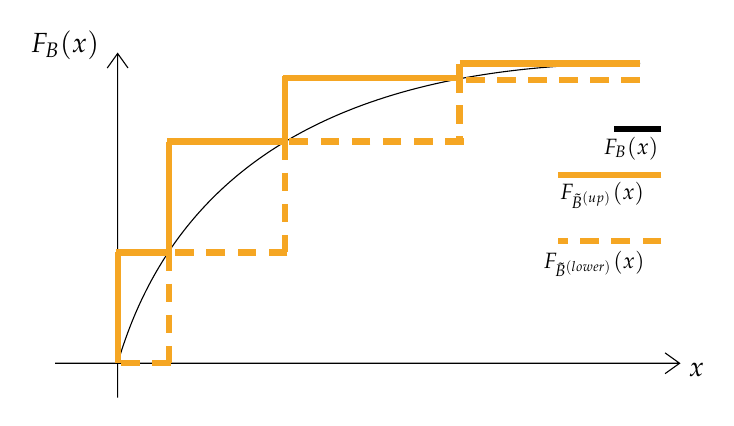
\begin{tikzpicture}[x=0.75pt,y=0.75pt,yscale=-1,xscale=1]
%uncomment if require: \path (0,300); %set diagram left start at 0, and has height of 300

%Shape: Axis 2D [id:dp0917203973178844] 
\draw  (48,194.42) -- (348.83,194.42)(78.08,45.17) -- (78.08,211) (341.83,189.42) -- (348.83,194.42) -- (341.83,199.42) (73.08,52.17) -- (78.08,45.17) -- (83.08,52.17)  ;
%Curve Lines [id:da8046234326772914] 
\draw    (78.08,194.42) .. controls (111.83,79) and (218.83,50) .. (329.83,50) ;
%Straight Lines [id:da9849769243307844] 
\draw [color={rgb, 255:red, 245; green, 166; blue, 35 }  ,draw opacity=1 ][line width=2.25]    (78.08,194.42) -- (78.08,141) ;
%Straight Lines [id:da3943481861674383] 
\draw [color={rgb, 255:red, 245; green, 166; blue, 35 }  ,draw opacity=1 ][line width=2.25]    (77.08,141) -- (102.83,141) ;
%Straight Lines [id:da008525076806593201] 
\draw [color={rgb, 255:red, 245; green, 166; blue, 35 }  ,draw opacity=1 ][line width=2.25]    (101.83,87.58) -- (158.83,87.58) ;
%Straight Lines [id:da6431146537588102] 
\draw [color={rgb, 255:red, 245; green, 166; blue, 35 }  ,draw opacity=1 ][line width=2.25]    (102.83,141) -- (102.83,87.58) ;
%Straight Lines [id:da052276646032704654] 
\draw [color={rgb, 255:red, 245; green, 166; blue, 35 }  ,draw opacity=1 ][line width=2.25]    (157.83,57) -- (242.83,57) ;
%Straight Lines [id:da6176137521249536] 
\draw [color={rgb, 255:red, 245; green, 166; blue, 35 }  ,draw opacity=1 ][line width=2.25]    (158.83,87.58) -- (158.83,56) ;
%Straight Lines [id:da19336635837959326] 
\draw [color={rgb, 255:red, 245; green, 166; blue, 35 }  ,draw opacity=1 ][line width=2.25]  [dash pattern={on 6.75pt off 4.5pt}]  (242.83,55) -- (242.83,87.58) ;
%Straight Lines [id:da8496050407473881] 
\draw [color={rgb, 255:red, 245; green, 166; blue, 35 }  ,draw opacity=1 ][line width=2.25]  [dash pattern={on 6.75pt off 4.5pt}]  (244.83,87.58) -- (158.83,87.58) ;
%Straight Lines [id:da3615064269180923] 
\draw [color={rgb, 255:red, 245; green, 166; blue, 35 }  ,draw opacity=1 ][line width=2.25]  [dash pattern={on 6.75pt off 4.5pt}]  (159.83,141) -- (102.83,141) ;
%Straight Lines [id:da8589349231177894] 
\draw [color={rgb, 255:red, 245; green, 166; blue, 35 }  ,draw opacity=1 ][line width=2.25]  [dash pattern={on 6.75pt off 4.5pt}]  (158.83,87.58) -- (158.83,141) ;
%Straight Lines [id:da45656775847848285] 
\draw [color={rgb, 255:red, 245; green, 166; blue, 35 }  ,draw opacity=1 ][line width=2.25]  [dash pattern={on 6.75pt off 4.5pt}]  (103.83,194.42) -- (78.08,194.42) ;
%Straight Lines [id:da23540563287937655] 
\draw [color={rgb, 255:red, 245; green, 166; blue, 35 }  ,draw opacity=1 ][line width=2.25]  [dash pattern={on 6.75pt off 4.5pt}]  (102.83,141) -- (102.83,194.42) ;
%Straight Lines [id:da7725424623835695] 
\draw [color={rgb, 255:red, 245; green, 166; blue, 35 }  ,draw opacity=1 ][line width=2.25]    (242.83,50) -- (329.83,50) ;
%Straight Lines [id:da4368156230854221] 
\draw [color={rgb, 255:red, 245; green, 166; blue, 35 }  ,draw opacity=1 ][line width=2.25]    (242.83,58) -- (242.83,50) ;
%Straight Lines [id:da055576776802613415] 
\draw [color={rgb, 255:red, 245; green, 166; blue, 35 }  ,draw opacity=1 ][line width=2.25]  [dash pattern={on 6.75pt off 4.5pt}]  (329.83,58) -- (243.83,58) ;
%Straight Lines [id:da6827425172306525] 
\draw [line width=2.25]    (340,81.58) -- (317.17,81.58) ;
%Straight Lines [id:da3881977243224537] 
\draw [color={rgb, 255:red, 245; green, 166; blue, 35 }  ,draw opacity=1 ][line width=2.25]    (340,103.58) -- (290,103.58) ;
%Straight Lines [id:da38195740555775237] 
\draw [color={rgb, 255:red, 245; green, 166; blue, 35 }  ,draw opacity=1 ][line width=2.25]  [dash pattern={on 6.75pt off 4.5pt}]  (340,135.58) -- (290,135.58) ;

% Text Node
\draw (35,33) node [anchor=north west][inner sep=0.75pt]   [align=left] {$\displaystyle F_{B}( x)$};
% Text Node
\draw (352,193) node [anchor=north west][inner sep=0.75pt]   [align=left] {$\displaystyle x$};
% Text Node
\draw (290,106) node [anchor=north west][inner sep=0.75pt]  [font=\footnotesize] [align=left] {$\displaystyle F_{\tilde{B}^{(up)}}( x)$};
% Text Node
\draw (282,139) node [anchor=north west][inner sep=0.75pt]  [font=\footnotesize] [align=left] {$\displaystyle F_{\tilde{B}^{(lower)}}( x)$};
% Text Node
\draw (311,84) node [anchor=north west][inner sep=0.75pt]  [font=\footnotesize] [align=left] {$\displaystyle F_{B}( x)$};
\end{tikzpicture}
\end{center}


\paragraph{Note}	Pour comprendre ce que représente le pas de discrétisation, voir la page 21 des diapositives sur les méthodes d'agrégation pour un excellent visuel.


\subsubsection{Méthodes de dispersion de la masse avec espérance préservée}
\paragraph{Note}	Ne semble pas être dans le cadre du cours pour l'automne 2020.

\bigskip

\begin{definitionNOHFILLpropos}[Lemme]
Soit les scalaires $a, b, c, d$ tels que :
\begin{itemize}
	\item	\lfbox[conditions]{$a < b$}
	\item	\lfbox[conditions]{$a < d < b$}
	\item	\lfbox[conditions]{$0 \leq c < 1$}
	\item	\lfbox[conditions]{$p_{a}, p_{b} \geq 0$}
\end{itemize}

Alors la solution au système de deux équations avec les deux inconnus suivants : 
\begin{align*}
	p_{a}	+	p_{b}	&=	c	\\
	ap_{a}	+	bp_{b}	&=	d
\end{align*}
est \lfbox[formula]{$p_{a}	=	\frac{bc	-	d}{b	-	a}$} et \lfbox[formula]{$p_{b}	=	\frac{d	-	ac}{b	-	a}$}.
\end{definitionNOHFILLpropos}

\begin{definitionNOHFILLprop}[Méthode de dispersion de la masse]
\setlength{\mathindent}{-1cm}
\begin{align*}
	p^{-}_{kh}
	&=	\frac{(k + 1)h}{h} \left\{
			F_{B}((k + 1)h)	-	F_{B}(kh)
		\right\}		\\	&\quad\quad	-	\frac{1}{h} \left\{
			\text{E}[B \times \bm{1}_{(-\infty, (k + 1)h]}]	-	\text{E}[B \times \bm{1}_{(-\infty, kh]}]	
		\right\}	\\
	p^{+}_{(k + 1)h}
	&=	\frac{1}{h} \left\{
			\text{E}[B \times \bm{1}_{(-\infty, (k + 1)h]}]	-	\text{E}[B \times \bm{1}_{(-\infty, kh]}]
		\right\}			\\	&\quad\quad -\frac{kh}{h} \left\{
			F_{B}((k + 1)h)	-	F_{B}(kh)
		\right\}		\\
\end{align*}

Puis on obtient que pour \lfbox[conditions]{$k \in \mathbb{N}^{+}$} \lfbox[formula]{$f_{\tilde{B}}(kh)	=	p^{+}_{kh} + p^{-}_{kh}$}. C'est-à-dire, 
\begin{align*}
	f_{\tilde{B}}(kh)
	&=	...
	=	\frac{1}{h}	\bigg\{
		2\text{E}[\min(B; kh)]	-	\text{E}[\min(B; (k - 1)h)]		-	\text{E}[\min(B; (k + 1)h)]	
		\bigg\}
\end{align*}
\setlength{\mathindent}{1cm}

Avec comme point de départ \lfbox[conditions]{$f_{\tilde{B}}(0)	=	1	-	\frac{\text{E}[\min(B; h)]}{h}$}.

\end{definitionNOHFILLprop}



\columnbreak
\subsection{Agrégation et transformée de Fourier rapide}
\begin{align*}
	\varphi_{X}(t_{j})
	&=	\text{E}[\textrm{e}^{it_{j}X}]
	=	\text{E}[\cos(t_{j}X)] + i \times \text{E}[\sin(t_{j}X)]	\\
	&=	\sum_{u = 0}^{n - 1} f_{X}(u) \textrm{e}^{i (2\pi) (j / n) u}
\end{align*}
où \lfbox[conditions]{$t_{j}	=	i2\pi(j/n)$}.

Également, \lfbox[formula]{$f_{X}(l)	=	\frac{1}{n} \sum_{j = 0}^{n - 1} \varphi(2\pi(j/n))\textrm{e}^{-i2\pi (j/n)l}$}.



\columnbreak
\subsection{Transformée de Fourier rapide}

\begin{algo2}[Somme de deux v.a. discrètes indépendantes]
Soit les v.a. discrètes $X$ et $Y$ avec la v.a. $S	=	X + Y$.	\\
Pour calculer la fonction de masse de probabilité $f_{S}$ de la v.a. $S$, les étapes sont les suivantes :
\begin{enumerate}
	\item	Construire les vecteurs $\underline{f}_{X}$ et $\underline{f}_{Y}$.
		\begin{itemize}
		\item	Ils doivent être d'une même longueur $2^{m}$.
		\item	Pour faire ceci, on ajoute des 0 aux vecteurs.
		\end{itemize}
	\item	Utiliser la fonction \texttt{fft} pour produire les vecteurs $\underline{\widetilde{f}}_{X}$ et $\underline{\widetilde{f}}_{Y}$ de $\underline{f}_{X}$ et $\underline{f}_{Y}$.
	\item	Faire le produit des deux vecteurs pour obtenir $\underline{\widetilde{f}}_{S}	=	\underline{\widetilde{f}}_{X} \times \underline{\widetilde{f}}_{Y}$.	
		\begin{itemize}
		\item	Ceci équivaut à une multiplication de vecteurs colonnes et donc le $i^{\text{e}}$ élément de $\underline{\widetilde{f}}_{X}$ multiplie le $i^{\text{e}}$ élément de $\underline{\widetilde{f}}_{Y}$.
		\end{itemize}
	\item	Utiliser la fonction \texttt{fft} avec \texttt{inverse = TRUE} pour produire le vecteur $\underline{f}_{S}$ de $\underline{\widetilde{f}}_{S}$.
		\begin{itemize}
		\item	On utilise la fonction \texttt{Re} pour conserver uniquement la partie réelle du chiffre.
		\item	Il faut diviser par $2^{m}$ pour obtenir les densités.
		\end{itemize}
\end{enumerate}
\end{algo2}

\begin{algo2}[Somme de $n$ v.a. discrètes indépendantes]
Soit les v.a. discrètes $X_{1}, \dots, X_{n}$ définies sur $\{0, 1h, 2h, \dots\}$ avec la v.a. $S	=	\sum_{i = 1}^{n} X_{i}$.\\
Pour calculer la fonction de masse de probabilité $f_{S}$ de la v.a. $S$, les étapes sont les suivantes :
\begin{enumerate}
	\item	Construire les vecteurs $\underline{f}_{X_{1}}, \dots, \underline{f}_{X_{n}}$.
		\begin{itemize}
		\item	Ils doivent être d'une même longueur $2^{m}$.
		\item	Pour faire ceci, on ajoute des 0 aux vecteurs.
		\end{itemize}
	\item	Utiliser la fonction \texttt{fft} pour produire les vecteurs $\underline{\widetilde{f}}_{X_{1}}, \dots, \underline{\widetilde{f}}_{X_{n}}$ de $\underline{f}_{X_{1}}, \dots, \underline{f}_{X_{n}}$.
	\item	Faire le produit des $n$ vecteurs pour obtenir $\underline{\widetilde{f}}_{S}	=	\underline{\widetilde{f}}_{X_{1}} \times \dots \times \underline{\widetilde{f}}_{X_{n}}$.	
	\item	Utiliser la fonction \texttt{fft} avec \texttt{inverse = TRUE} pour produire le vecteur $\underline{f}_{S}$ de $\underline{\widetilde{f}}_{S}$ en conservant la partie réelle avec \texttt{Re} puis divisant par $2^{m}$.
\end{enumerate}
\end{algo2}

\begin{algo2}[Somme aléatoire (loi composée)]
Soit la v.a. composée $X$ avec $X	=	B_{1}	+	\dots	+	B_{M}$ si $M	> 0$ ou $X = 0$ si $M	=	0$ (et les hypothèses habituelles). \\
On pose que les v.a. $B_{1}, B_{2}, \dots$ sont définies sur $\{0, 1h, 2h, \dots\}$.
Pour calculer la fonction de masse de probabilité $f_{X}$ de la v.a. $X$, les étapes sont les suivantes :
\begin{enumerate}
	\item	Construire le vecteur $\underline{f}_{B}$.
		\begin{itemize}
		\item	Ajouter des 0 au vecteur pour qu'il soit d'une longueur de $2^{m}$.
		\end{itemize}
	\item	Utiliser la fonction \texttt{fft} pour produire le vecteur $\underline{\widetilde{f}}_{B}$ de $\underline{f}_{B}$.
	\item	Trouver le vecteur $\underline{\widetilde{f}}_{X}	=	\mathcal{P}_{M}(\underline{\widetilde{f}}_{B})$.
	\item	Utiliser la fonction \texttt{fft} avec \texttt{inverse = TRUE} pour produire le vecteur $\underline{f}_{X}$ de $\underline{\widetilde{f}}_{X}$ en conservant la partie réelle avec \texttt{Re} puis divisant par $2^{m}$.
\end{enumerate}
\end{algo2}


%\columnbreak
%\subsection{Distribution mélange d'Erlang}



\pagebreak
\section{Comparaison des risques et ordres stochastiques}


\pagebreak
\section{Distributions multivariées et agrégation des risques}
\begin{rappel_enhanced}[Contexte]
Il est devenu crucial de tenir compte de la dépendance dans les modélisations d'un portefeuille de risques.
\begin{itemize}
	\item	Il existe pour chaque loi paramétrique (discrète ou continue) plusieurs extensions multivariées.
	\item	Des lois multivariées peuvent être créées en se basant sur la théorie des copules.
	\item	Il existe des différentes approches pour construire des modèles multivariés de risque: 
		\begin{itemize}
		\item	modèles avec chocs communs,
		\item	modèles avec mélange commun,
		\item	etc.
		\end{itemize}
\end{itemize}
\end{rappel_enhanced}


\subsection{Classes de Fréchet}
Soit : 
\begin{itemize}
	\item	Des fonctions de répartition univariées (pas nécessairement identiques) $F_{1}, \dots, F_{n}$.
	\item	Le vecteur de v.a. $\underline{X}	=	(X_{1}, \dots, X_{n})$ dont la fonction de répartition est $F_{\underline{X}}$.
\end{itemize}
\begin{definitionNOHFILL}[Classe de Fréchet $\mathcal{CF}(F_{1}, \dots, F_{n})$]
Ensemble de toutes les fonctions de répartition multivariées $F_{\underline{X}}$ ayant pour marginales $F_{1}, \dots, F_{n}$.
\end{definitionNOHFILL}

\begin{definitionNOHFILLprop}[Théorème 13.2]

Soit : 
\begin{itemize}
	\item	$W(x_{1}, \dots, x_{n})	=	\max\left(\sum_{i = 1}^{n} F_{i}(x_{i}) - (n - 1); 0\right)$.
		\begin{itemize}
		\item	Ceci correspond à la borne inférieure de Fréchet et est une fonction de répartition si $n = 2$.
		\end{itemize}
	\item	$M(x_{1}, \dots, x_{n})	=	\min\left(F_{1}(x_{1}); \dots; F_{n}(x_{n})\right)$.
		\begin{itemize}
		\item	Ceci correspond à la borne supérieure de Fréchet et est une fonction de répartition.
		\end{itemize}
	\item	$F_{\underline{X}} \in \mathcal{CF}(F_{1}, \dots, F_{n})$.
\end{itemize}

Alors \lfbox[formula]{$W(x_{1}, \dots, x_{n})	\leq	F_{\underline{X}}(x_{1}, \dots, x_{n})	\leq	M(x_{1}, \dots, x_{n})$} pour \lfbox[conditions]{$(x_{1}, \dots, x_{n}) \in \mathbb{R}^{n}$}. 
\end{definitionNOHFILLprop}

\bigskip

Également, pour $X_{1}, X_{2}$ où $F_{X_{1}, X_{2}} \in \mathcal{CF}(F_{1}, F_{2})$, 
\begin{enumerate}
	\item	\lfbox[formula]{$\text{Cov}(X_{1}^{\min}, X_{2}^{\min}) \leq \text{Cov}(X_{1}, X_{2}) \leq \text{Cov}(X_{1}^{\max}, X_{2}^{\max})$}.
	\item	\lfbox[formula]{$-1 \leq \rho_{P}(X_{1}^{\min}, X_{2}^{\min}) \leq \rho_{P}(X_{1}, X_{2}) \leq \rho_{P}(X_{1}^{\max}, X_{2}^{\max}) \leq 1$}.
\end{enumerate}




\columnbreak
\subsection{Notions de dépendance}
\subsubsection{L'indépendance}
La notion de dépendance avec laquelle nous sommes familiers est l'indépendance.
\begin{definitionNOHFILLprop}[Indépendance]
Pour \lfbox[conditions]{$(x_{1}, x_{2}, \dots, x_{n}) \in \mathbb{R}^{n}$},
\begin{align*}
	F_{X_{1}, X_{2}, \dots, X_{n}}(x_{1}, x_{2}, \dots, x_{n})
	&=	F_{X_{1}}(x_{1}) \times \dots \times F_{X_{n}}(x_{n})
\end{align*}
\end{definitionNOHFILLprop}

\subsubsection{Comonotonicité}
La comonotonicité est un cas particulier de relation de dépendance. Elle correspond à la relation de dépendance positive parfaite.
\begin{definitionNOHFILLprop}[Comonotonicité]
Le vecteur de v.a. $\underline{X}	=	(X_{1}, X_{2}, \dots, X_{n})$ est comonotonique ssi il existe une v.a. $Z$ et des fonctions non décroissantes $\phi_{1}, \phi_{2}, \dots, \phi_{n}$ telles que :
\begin{align*}
	\underline{X}	
	=	(X_{1}, X_{2}, \dots, X_{n})
	&\overset{d}{=}	\phi_{1}(Z), \phi_{2}(Z), \dots, \phi_{n}(Z)
\end{align*}
\begin{itemize}
	\item	C'est à dire, le vecteur est comonotonique ssi ses composantes sont comonotones.
	\item	Les composante sont comonotones ssi la fonction de répartition conjointe du vecteur est la borne supérieure de Fréchet $M$.
\end{itemize}
\end{definitionNOHFILLprop}

\begin{algo2}[Simulation des réalisations d'un vecteur de v.a. comonotone]
Soit le vecteur de v.a. comonotones $\underline{X}	=	(X_{1}, X_{2}, \dots, X_{n})$.
\begin{enumerate}
	\item	On simule une réalisation $U^{(j)}$ d'une loi $U(0, 1)$.
	\item	On calcule le vecteur de réalisations $X^{(j)}_{1}	=	F_{X_{1}}^{-1}(U^{(j)}), \dots, X^{(j)}_{n}	=	F_{X_{n}}^{-1}(U^{(j)})$.
\end{enumerate}
\end{algo2}

\begin{definitionNOHFILLpropos}[Additivité des mesures de risque]
Soit un vecteur de v.a. comonotones $\underline{X}	=	(X_{1}, X_{2}, \dots, X_{n})$ et $S	=	\sum_{i = 1}^{n} X_{i}$.
Alors, $S	=	\sum_{i = 1}^{n}F_{X_{i}}^{-1}(U)	=	\phi(U)$.
\begin{align*}
	VaR_{\kappa}(S)	
	&=	\sum_{i = 1}^{n} VaR_{\kappa}(X_{i})	\\
	TVaR_{\kappa}(S)	
	&=	\sum_{i = 1}^{n} TVaR_{\kappa}(X_{i})
\end{align*}

Et 
\begin{align*}
	\text{E}[S \times \bm{1}_{\{S > d\}}]	
	&=	\sum_{i = 1}^{n} \int_{\phi^{-1}(d)}^{1} F^{-1}_{X_{i}}(u) du
\end{align*}
\end{definitionNOHFILLpropos}



\subsubsection{Antimonotonicité}
L'antimonotonicité correspond à la relation de dépendance \textbf{négative} parfaite définie pour des paires de v.a.

\begin{definitionNOHFILLprop}[Antimonotonicité]
Les composantes du couple de v.a. $\underline{X}	=	(X_{1}, X_{2})$ sont antimonotoniques ssi il existe une v.a. $Z$, une fonctions croissante $\phi_{1}$ et une fonction décroissantes $\phi_{2}$  telles que :
\begin{align*}
	(X_{1}, X_{2})
	&\overset{d}{=}	\left(\phi_{1}(Z), \phi_{2}(Z)\right)
\end{align*}
\begin{itemize}
	\item	Donc, si la fonction de répartition conjointe est la borne inférieure de Fréchet $F^{-}_{X_{1}, X_{2}}$.
\end{itemize}
\end{definitionNOHFILLprop}

\begin{algo2}[Simulation des réalisations d'un couple de v.a. antimonotones]
Soit le couple de v.a. antimonotones $(X_{1}, X_{2})$.
\begin{enumerate}
	\item	On simule une réalisation $U^{(j)}$ d'une loi $U(0, 1)$.
	\item	On calcule le vecteur de réalisations $X^{(j)}_{1}	=	F_{X_{1}}^{-1}(U^{(j)}), X^{(j)}_{2}	=	F_{X_{2}}^{-1}(1 - U^{(j)})$.
\end{enumerate}
\end{algo2}

\columnbreak
\subsubsection{Notation}
\begin{distributions}[Notation]
\begin{description}
	\item[$(X_{1}^{+}, X_{2}^{+})$]	Couple de v.a. comonotones avec \lfbox[formula]{$F_{X_{1}^{+}, X_{2}^{+}}(x_{1}, x_{2})	=	M(x_{1}, x_{2})	=	\min\left(F_{1}(x_{1}); F_{2}(x_{2})\right)$}.
	\item[$(X_{1}^{-}, X_{2}^{-})$]	Couple de v.a. antimonotones avec \lfbox[formula]{$F_{X_{1}^{-}, X_{2}^{-}}(x_{1}, x_{2})	=	W(x_{1}, x_{2})	=	\max\left(F_{1}(x_{1}) + F_{2}(x_{2}) - 1; 0\right)$}.
	\item[$(X_{1}^{\perp}, X_{2}^{\perp})$]	Couple de v.a. indépendantes avec \lfbox[formula]{$F_{X_{1}^{\perp}, X_{2}^{\perp}}(x_{1}, x_{2})	=	F_{1}(x_{1}) \times F_{2}(x_{2})$}.
\end{description}
\end{distributions}

\begin{distributions}[Notation]
\begin{description}
	\item[$\Delta_{a_{i}, b_{i}}F_{\underline{X}}(\underline{x})$]	$F_{\underline{X}}(x_{1}, \dots, b_{i}, \dots, x_{n})	-	F_{\underline{X}}(x_{1}, \dots, a_{i}, \dots, x_{n})$.
		\begin{itemize}
		\item	Pour $n = 2$, $\Pr(\underline{a}	<	X	\leq		b)	=	\Delta_{a_{1}, b_{1}}\Delta_{a_{2}, b_{2}} F_{\underline{X}}(\underline{x})	=	F_{\underline{X}}(b_{1}, b_{2}) - F_{\underline{X}}(a_{1}, b_{2}) - F_{\underline{X}}(b_{1}, a_{2}) + F_{\underline{X}}(a_{1}, a_{2})$.
		\end{itemize}
\end{description}
\end{distributions}


On peut déduire que pour $S = \sum_{i = 1}^{n} X_{i}$ où $F_{\underline{X}}(x_{1}, \dots, x_{n}) \leq F_{\underline{X}^{+}}(x_{1}, \dots, x_{n})$, alias $F_{\underline{X}} \in \mathcal{CF}(F_{1}, \dots, F_{n})$, 
\begin{enumerate}
	\item	$\text{E}[S] = \text{E}[S^{+}]$
	\item	$\text{Var}(S) \leq \text{Var}(S^{+})$.
	\item	$TVaR_{\kappa}(S) \leq TVaR_{\kappa}(S^{+})$.
	\item	$\text{E}[\max(S - d; 0)] \leq \text{E}[\max(S^{+} - d; 0)]$.
\end{enumerate}


\begin{definitionNOHFILLprop}[Proposition 7]
Soit la paire de v.a. continues $\underline{X} = (X_{1}, X_{2})$ dont $F_{X_{1}, X_{2}} \in \mathcal{CF}(F_{1}, F_{2})$ et dont $F_{1}(0) = F_{2}(0) = 0$. De plus, on pose que $X_{1} \sim X_{2} \sim X$, puis que $\phi(u) = F^{-1}(u) + F^{-1}(1 - u)$ est convexe pour $u \in (0, 1)$. 

\bigskip

Alors, \lfbox[formula]{$VaR_{\kappa}(X_{1}^{-} + X_{2}^{-}) = VaR_{\frac{1 - \kappa}{2}}(X) + VaR_{\frac{1 + \kappa}{2}}(X)$} et \lfbox[formula]{$TVaR_{\kappa}(X_{1}^{-} + X_{2}^{-}) = LVaR_{\frac{1 - \kappa}{2}}(X) + LVaR_{\frac{1 + \kappa}{2}}(X)$}.

\bigskip

La convexité de $\phi$ peut être confirmée en vérifiant que $\frac{\partial^{2}}{\partial x^{2}} \bar{F}(x) \geq 0$ pour $x \in \mathbb{R}^{+}$.

%De plus, il s'ensuit que pour $0 < u_{1} < 0.5 < u_{2}$, alors $\phi(u_{1}) = \phi(u_{2}) = x$ et que $F_{X_{1}^{-} + X_{2}^{-}}(x) = u_{2} - u_{1} = \kappa = 2\gamma$. Finalement, on déduit que \lfbox[formula]{$VaR_{\kappa}(X_{1}^{-} + X_{2}^{-}) = \phi\left(\frac{1}{2} - \frac{\kappa}{2}\right)$}
\end{definitionNOHFILLprop}

\bigskip

Si les v.a. $X_{1}, \dots, X_{n}$ sont indépendantes \lfbox[formula]{$\text{E}[g_{1}(X_{1}) \dots g_{n}(X_{n})] = \text{E}[g_{1}(X_{1})] \times \dots \times \text{E}[g_{n}(X_{n})]$}.



\columnbreak
\subsection{Loi multivariées}
\begin{definitionNOHFILL}[Loi de Poisson bivariée de Teicher]
Soit : 
\begin{itemize}
	\item	Le couple de v.a. $(M_{1}, M_{2})$ où $M_{i} \sim \text{pois}(\lambda_{i})$ pour $i	=	1, 2$.
	\item	Les v.a. indépendantes $K_{0}, K_{1}, K_{2}$ avec $K_{i}	\sim \text{Pois}(\alpha_{i})$ pour $i	=	0, 1, 2$ et $\alpha_{i}	=	\lambda_{i}	-	\alpha_{0}$ pour $i	=	1, 2$ où $0	\leq	\alpha_{0}	\leq	\min(\lambda_{1}, \lambda_{2})$.
\end{itemize}

\bigskip

On définit $M_{i}	=	K_{i} + K_{0}$ pour $i	=	1, 2$.
\begin{itemize}
	\item	$K_{i}$ représente la fréquence d'un \og choc \fg{} spécifique à la $i^{\text{e}}$ ligne d'affaires pour $i = 1, 2$.
	\item	$K_{0}$ représente la fréquence d'un \og choc \fg{} commun aux deux lignes d'affaires.
\end{itemize}

Donc, $(M_{1}, M_{2})	\sim \text{PBivTeicher}(\lambda_{1}, \lambda_{2}, \alpha_{0})$.
\end{definitionNOHFILL}



\columnbreak
\subsection{Lois composées multivariées}
%%%	----------------------------------------
%%%	je ne sais pas si ça vaut la peine d'inclure ceci :
%L'analogue de la relation récursive de la famille $(a, b, 0)$ pour le couple $(M_{1}, M_{2}) \sim \text{PBiv}(\lambda_{1}, \lambda_{2}, \alpha_{0})$ avec le point de départ \lfbox[formula]{$f_{M_{1}, M_{2}}(0, 0)	=	\textrm{e}^{-\lambda_{1} - \lambda_{2} + \alpha_{0}}$} pour :
%
%%\lfbox[conditions]{$m_{1} \in \mathbb{N}^{+}, m_{2}	=	0$}, est \lfbox[formula]{$f_{M_{1}, M_{2}}(m_{1}, m_{2})	=	\frac{\lambda_{1} - \alpha_{0}}{m_{1}}f_{M_{1}, M_{2}}(m_{1} - 1, 0)$}.
%
%\lfbox[conditions]{$m_{1} \in \mathbb{N}^{+}, m_{2}	\in \mathbb{N}^{+}$}, est \lfbox[formula]{$f_{M_{1}, M_{2}}(m_{1}, m_{2})	=	\frac{\lambda_{1} - \alpha_{0}}{m_{1}}f_{M_{1}, M_{2}}(m_{1} - 1, m_{2})$}\\ \lfbox[formula]{$+ \frac{\alpha_{0}}{m_{1}}f_{M_{1}, M_{2}}(m_{1} - 1, m_{2} - 1)$}. 
%%%	----------------------------------------

\begin{rappel}{Covariance totale}
\setlength{\mathindent}{-1cm}
\begin{align*}
    \text{Cov}(X_{1}, X_{2})
    &=  \text{E}_{M_{1}, M_{2}}\left[\text{Cov}(X_{1}, X_{2} | M_{1}, M_{2})\right] + \\ &\text{Cov}_{M_{1}, M_{2}}\left( \text{E}\left[X_{1}| M_{1}, M_{2}\right]\text{E}\left[X_{2}| M_{1}, M_{2}\right]\right)
\end{align*}
\setlength{\mathindent}{1cm}
\end{rappel}


\begin{definitionNOHFILL}[Loi Poisson composée]
Soit : 
\begin{itemize}
	\item	Les v.a. indépendantes $K_{0}, K_{1}, \dots, K_{n}$ avec :
		\begin{itemize}
		\item	\lfbox[formula]{$K_{0} \sim  \text{Pois}(\alpha_{0})$} pour \lfbox[conditions]{$0	\leq	\alpha_{0}	\leq	\min(\lambda_{1}; \dots; \lambda_{n})$}, 
		\item	\lfbox[formula]{$K_{i} \sim  \text{Pois}(\alpha_{i} = \lambda_{i} - \alpha_{0})$} pour \lfbox[conditions]{$i	=	1, 2, \dots, n$}.
		\end{itemize}
	\item	Le vecteur de v.a. de fréquence $(M_{1}, \dots, M_{n})$ obéit à une loi de Poisson multivariée de Teicher (avec choc commun). 
		\begin{itemize}
		\item	Les composantes du vecteur sont définies par $M_{i}	=	K_{i} + K_{0}$.
		\item	Alors, \lfbox[formula]{$M_{i}	\sim \text{Pois}(\lambda_{i})$}.
		\end{itemize}
	\item	Le vecteur de v.a. $(X_{1}, \dots, X_{n})$ obéit à une loi de Poisson composée multivariée.
\end{itemize}
Alors, \lfbox[formula]{$S	=	\sum_{i	=	1}^{n}X_{i}	\sim	\sim \text{PComp}(\lambda_{S}; F_{C})$} où :
\begin{itemize}
	\item	\lfbox[conditions]{$\lambda_{S}	=	\sum_{i	=	1}^{n}\lambda_{i}	-	(n - 1)\alpha_{0}$}.
	\item	\lfbox[conditions]{$F_{C}(x)	=	\sum_{i	=	1}^{n}\left\{\frac{\lambda_{i} - \alpha_{0}}{\lambda_{S}} F_{B_{i}}(x)\right\} + \frac{\alpha_{0}}{\lambda_{S}} F_{B_{1} + \dots + B_{n}}(x)$}.
\end{itemize}
\end{definitionNOHFILL}



\pagebreak 
\section{Théorie des copules}
\begin{definitionNOHFILL}[Famille de copules archimédiennes]
Une copule $C$ est dite « \textbf{archimédienne} » si elle s'écrit sous la forme \lfbox[formula]{$C(u_{1}, \dots, u_{n}) = \psi\left(\psi^{-1}(u_{1}) + \dots + \psi^{-1}(u_{n}\right)$}.	\\

La fonction $\psi$ est appelé « \textit{générateur} » et satisfait aux propriétés suivantes :
\begin{enumerate}[label	=	\circled{\arabic*}{trueblue}]
	\item	$\psi: [0, \infty) \rightarrow [0, 1]$ avec $\psi(0) = 1$ et $\lim_{x \rightarrow \infty} \psi(x) = 0$ ;
	\item	$\psi$ est une fonction continue ;
	\item	$\psi$ est une fonction strictement décroissante sur $[0, \infty)$ ;
	\item	$\psi^{-1}$ est la fonction inverse tel que $\psi^{-1} = \inf\{u, \psi(u) \leq x\}$.
\end{enumerate}
\end{definitionNOHFILL}


\begin{definitionNOHFILLsub}[Copule de Clayton]
Pour $i = 1, 2$, $u \in [0, 1]$ et $\alpha > 0$ :
\begin{align*}
	C_{\alpha}(u_{1}, u_{2})
	&=	\left(u_{1}^{-\alpha} + u_{2}^{-\alpha} - 1\right)^{-1/\alpha}	\\
	c_{\alpha}(u_{1}, u_{2})
	&=	\frac{1 + \alpha}{(u_{1}u_{2})^{\alpha + 1}} \left(u_{1}^{-\alpha} + u_{2}^{-\alpha} - 1\right)^{-2 - 1/\alpha}	
\end{align*}
\end{definitionNOHFILLsub}

\begin{definitionNOHFILLsub}[Copule de Gumbel]
Pour $i = 1, 2$, $u \in [0, 1]$ et $\alpha \geq 1$ :
\begin{align*}
	C_{\alpha}(u_{1}, u_{2})
	&=	\textrm{exp}\left\{-\left([-\ln(u_{1})]^{\alpha} + [-\ln(u_{2})]^{\alpha}\right)^{1/\alpha}\right\}	
\end{align*}
\end{definitionNOHFILLsub}


\newpage
\part{Autres}
\section{Terminologie}
\begin{description}
	\item[$\argmax$]	Si on pose que $\hat{\theta}	=	\argmax L(\theta; \bm{X})$ on dit que la valeur maximale de $L(\theta; \bm{X})$ est au point $\hat{\theta}$.
\end{description}

Paramètre
\begin{description}
%%%	https://www.statisticshowto.com/shape-parameter/
	\item[de forme]	Affecte la forme générale de la distribution;
		\begin{itemize}
		\item	\og \textit{shape parameter} \fg{};
		\item	Il est important de saisir que le paramètre de forme n'a aucune incidence sur l'emplacement de la densité (paramètre de l'emplacement) ni sur l'échelle de la densité (paramètre d'échelle);
		\item	Par exemple, la distribution Gamma a un paramètre de forme qui impact comment qu'elle est représentée;
		\item	Par exemple, la distribution exponentielle n'a pas de paramètre de forme et bien que l'échelle de la distribution peut être modifiée, la forme générale est constante.
		\end{itemize}
%%%		
	\item[d'échelle]	Sert à déterminer la forme et l'emplacement de la distribution en étirant ou compressant la densité;
		\begin{itemize}
		\item	\og \textit{scale parameter} \fg{};
		\item	Le plus gros le paramètre d'échelle, le plus rependue la distribution;
		\item	On peut voir ceci visuellement où avec un paramètre d'échelle de 1, la distribution est inchangée:
		\end{itemize}
		\begin{center}
\tikzset{every picture/.style={line width=0.75pt}} %set default line width to 0.75pt        

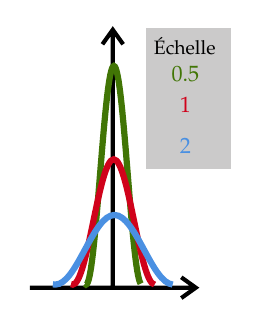
\begin{tikzpicture}[x=0.75pt,y=0.75pt,yscale=-1,xscale=1]
%uncomment if require: \path (0,300); %set diagram left start at 0, and has height of 300

%Shape: Axis 2D [id:dp18693685040272978] 
\draw [line width=1.5]  (119.83,151.67) -- (199.83,151.67)(159.83,27.4) -- (159.83,151.67) (192.83,146.67) -- (199.83,151.67) -- (192.83,156.67) (154.83,34.4) -- (159.83,27.4) -- (164.83,34.4)  ;
%Shape: Wave [id:dp5641937191696826] 
\draw  [color={rgb, 255:red, 65; green, 117; blue, 5 }  ,draw opacity=1 ][line width=2.25]  (146.41,149.77) .. controls (146.59,150.04) and (146.77,150.18) .. (146.95,150.18) .. controls (149.38,150.18) and (151.47,124.5) .. (153.66,97.51) .. controls (155.85,70.53) and (157.94,44.84) .. (160.37,44.84) .. controls (162.8,44.84) and (164.89,70.53) .. (167.08,97.51) .. controls (169.1,122.49) and (171.05,146.35) .. (173.25,149.77) ;
%Shape: Wave [id:dp9736357574926828] 
\draw  [color={rgb, 255:red, 208; green, 2; blue, 27 }  ,draw opacity=1 ][line width=2.25]  (139.7,149.94) .. controls (139.97,150.1) and (140.23,150.18) .. (140.5,150.18) .. controls (144.08,150.18) and (147.17,135.46) .. (150.39,119.99) .. controls (153.62,104.52) and (156.71,89.8) .. (160.29,89.8) .. controls (163.87,89.8) and (166.96,104.52) .. (170.19,119.99) .. controls (173.38,135.28) and (176.43,149.85) .. (179.96,150.18) ;
%Shape: Wave [id:dp9806953027168039] 
\draw  [color={rgb, 255:red, 74; green, 144; blue, 226 }  ,draw opacity=1 ][line width=2.25]  (130.98,150.05) .. controls (131.36,150.14) and (131.74,150.18) .. (132.12,150.18) .. controls (137.28,150.18) and (141.73,142) .. (146.38,133.41) .. controls (151.03,124.82) and (155.48,116.64) .. (160.64,116.64) .. controls (165.8,116.64) and (170.25,124.82) .. (174.9,133.41) .. controls (179.4,141.74) and (183.72,149.68) .. (188.68,150.16) ;
%Shape: Rectangle [id:dp4682062525043522] 
\draw  [draw opacity=0][fill={rgb, 255:red, 203; green, 202; blue, 202 }  ,fill opacity=1 ] (176,26.67) -- (216.83,26.67) -- (216.83,94.67) -- (176,94.67) -- cycle ;

% Text Node
\draw (178.42,29.67) node [anchor=north west][inner sep=0.75pt]  [font=\scriptsize,color={rgb, 255:red, 0; green, 0; blue, 0 }  ,opacity=1 ] [align=left] {Échelle};
% Text Node
\draw (186.92,43.67) node [anchor=north west][inner sep=0.75pt]  [font=\footnotesize,color={rgb, 255:red, 65; green, 117; blue, 5 }  ,opacity=1 ] [align=left] {0.5};
% Text Node
\draw (190.92,58.67) node [anchor=north west][inner sep=0.75pt]  [font=\footnotesize,color={rgb, 255:red, 208; green, 2; blue, 27 }  ,opacity=1 ] [align=left] {1};
% Text Node
\draw (190.92,78.67) node [anchor=north west][inner sep=0.75pt]  [font=\footnotesize,color={rgb, 255:red, 74; green, 144; blue, 226 }  ,opacity=1 ] [align=left] {2};


\end{tikzpicture}
		\end{center}
	\item[de fréquence]	L'interprétation dépend du contexte.
		\begin{itemize}
		\item	\og \textit{rate parameter} \fg{};
		\item	Dans le cas d'un processus de Poisson, le paramètre de fréquence décrit le taux auquel les événements se produisent;
		\item	Souvent, il est défini comme le réciproque du paramètre d'échelle pour indiquer le taux de déclin d'une fonction exponentielle;
		\item	Des valeurs près de 1 impliquent un déclin lent alors que des valeurs près de 0 impliquent un déclin rapide.
		\end{itemize}
%%%		https://www.statisticshowto.com/location-parameter/
	\item[d'emplacement]	Stipule où la densité est située.
		\begin{itemize}
		\item	\og \textit{location parameter} \fg{};
		\item	Plus précisément, indique où sur l'axe des $x$ la distribution est centrée relatif à la distribution normale standard;
		\item	Une distribution normale standard est centrée à 0 donc un paramètre d'emplacement de 5 implique que la densité est centrée à $x	=	5$.
		\end{itemize}
\end{description}


\begin{distributions}[Notation]
\begin{description}
	\item[$S$]	Les coûts d'un portefeuille.
	\item[$\rho(S)$]	Une mesure de risque.
\end{description}
\end{distributions}



\pagebreak

\section{Preuves}

\subsection*{\hypertarget{proof:ftc-quantile}{Preuve du théorème de la fonction quantile}}
\begin{formula}{}
\begin{align*}
	F_{F_{X}^{-1}(U)}
	&=	\Pr\left(F_{X}^{-1}(U) \leq x\right)	\\
	&\overset{2}{=}	\Pr\left(U \leq F_{X}(x)\right)	\\
	&\overset{1}{=}	F_{X}(x)
\end{align*}
\begin{enumerate}
	\item	Pour $U \sim Unif(0, 1)$, $F_{U}(u)	=	\Pr(U	\leq	u)	=	u$ alors $F_{U}(F_{X}(x))	=	F_{X}(x)$.
	\item	On doit prouver que:
		\begin{align*}
		\bigg\{	F_{X}^{-1}(U)	\leq	x	\bigg\}
		=
		\bigg\{	U	\leq	F_{X}(x)	\bigg\}
		\end{align*}
\end{enumerate}

\tcbline

\paragraph{Cas 1:	$X$ est une variable aléatoire continue}
\begin{itemize}
	\item	Alors, l'équivalence est vraie puisque $\{	F_{X}^{-1}(U)	\leq	x	\}$ est la solution unique à $\{	U	\leq	F_{X}(x)	\}$ par définition.
\end{itemize}

\paragraph{Cas 2:	$X$ est une variable aléatoire quelconque}
\begin{enumerate}
	\item	On fixe \lfbox[conditions]{$x	=	F_{X}^{-1}(u)	=	\inf\{y \in \mathbb{R}; F_{X}(y)	\geq u\}$} ;
		\begin{itemize}
		\item	Donc, ce "$x$" est une valeur parmi les valeurs "$y$" qui rencontre la condition $F_{X}(y)	\geq	u$ ;
		\item	Il s'ensuit que puisque $u \leq F_{X}(y)$ alors \lfbox[conditions]{$u \leq F_{X}(x)$}.
		\end{itemize}
		\begin{align*}
		\bigg\{	F_{X}^{-1}(U)	\leq	x	\bigg\}
		\Rightarrow
		\bigg\{	U	\leq	F_{X}(x)	\bigg\}
		\end{align*}
	\item	On fixe \lfbox[conditions]{$u \leq F_{X}(x)$} ;
		\begin{itemize}
		\item	Puisque la fonction quantile est la plus petite valeur de $y$ tel que $u \leq F_{X}(y)$, il s'ensuit que $F_{X}^{-1}(u)	\leq  x$.
		\end{itemize}
		\begin{align*}
		\bigg\{	U	\leq	F_{X}(x)	\bigg\}
		\Rightarrow
		\bigg\{	F_{X}^{-1}(U)	\leq	x	\bigg\}
		\end{align*}
\end{enumerate}
Donc :
\begin{align*}
	\bigg\{	F_{X}^{-1}(U)	\leq	x	\bigg\}
	=
	\bigg\{	U	\leq	F_{X}(x)	\bigg\}
\end{align*}
\end{formula}


\subsection*{\hypertarget{proof:stoploss}{Preuve de la fonction Stop-Loss comme la survie}}
\begin{enumerate}
	\item	Premièrement, on développe l'expression :
		\begin{align}
		\pi_{X}(d)
			&=	\text{E}[\max(X - d; 0)]	\nonumber\\
			&=	\int_{-\infty}^{\infty} {\color{teal}\max(x - d; 0)} f_{X}(x)dx	\nonumber\\
			&=	\int_{-\infty}^{d} {\color{teal}(0)} f_{X}(x)dx	+	\int_{d}^{\infty} {\color{teal}(x - d)} {\color{amethyst}f_{X}(x)}dx	\nonumber\\
			&=	\int_{d}^{\infty} {\color{teal}(x - d)} f_{X}(x)dx	
%			&=	\int_{d}^{\infty} (x - d) \left({\color{amethyst}\deriv{x}{F_{X}(x)}}\right)dx	
		\end{align}
\end{enumerate}

Pour la prochaine étape, nous avons recours au théorème des accroissements finis :
\begin{rappel_enhanced}[Théorème des accroissements finis]
Soit la fonction $f$ qui répond aux critères suivants :
\begin{enumerate}
	\item	$f(x)$ est continue sur l'intervalle fermé $[a, b]$ ;
	\item	$f(x)$ est différentiable sur l'intervalle ouvert $(a, b)$.
\end{enumerate}

Alors, il existe un nombre $c$ tel que \lfbox[conditions]{$a < c < b$} et \lfbox[formula]{$f'(c)	=	\frac{f(b) - f(a)}{b - a}$}.
\end{rappel_enhanced}

De plus, nous avons recours à l'intégrale de Riemann-Stieltjes :

\begin{rappel_enhanced}[Intégrale de Riemann-Stieltjes]
Sois les fonctions $f$ et $g$ continues sur l'intervalle $[a, b]$.
\begin{itemize}
	\item	On divise l'ensemble $[a, b]$ en $n$ sous-intervalles $c_{i} = [x_{i - 1}, x_{i}]$.
	\item	Les $n$ partitions $P$ des sous-intervalles sont aux points $P	=	\{a	=	x_{0} < x_{1} < \hdots < x_{n} = b\}$. 
	\item	La norme des partitions est la longueur du plus long sous-intervalle $\lVert P \rVert	=	\underset{1 \leq i \leq n}{\max}\{|x_{i} - x_{i - 1}|\}$.
	\item	On dénote le $i^{\text{e}}$ point du sous-intervalle $c_{i}$ par $t_{i} \in [x_{i - 1}, x_{i}]$.
\end{itemize}

On obtient donc l'intégrale de Riemann : \lfbox[formula]{$\limz{\lVert P \rVert}{0}\ \sumz{n}{i = 1} f(t_{i})(x_{i} - x_{i - 1})	=	\int_{a}^{b}f(x)dx$}.\\

L'intégrale de Riemann-\textit{Stieltjes} généralise l'intégrale de Riemann avec une fonction $g$ comme mesure de distance entre les points $x_{i - 1}$ et $x_{i}$; l'intégrale de Riemann-Stieltjes est donc : \lfbox[formula]{$\limz{\lVert P \rVert}{0}\ \sumz{n}{i = 1} f(t_{i})(g(x_{i - 1}) - g(x_{i}))	=	\int_{a}^{b}f(x)dg(x)$}.
\end{rappel_enhanced}


\begin{enumerate}[resume]
	\item	On réécrit \textbf{l'intégrale indéfinie} avec une limite afin d'obtenir un intervalle borné :
		\begin{align}
		\int_{d}^{\infty} (x - d) f(x) dx
			&=	\limz{{\color{cyan}c}}{\infty} \int_{d}^{{\color{cyan}c}} (x - d) f(x) dx	
		\end{align}
	\item	On réécrit l'intégrale sous la forme de \textbf{l'intégrale de Riemann} :
		\begin{align}
		\limz{c}{\infty} \int_{d}^{c} (x - d) f(x) dx	
			&=	\limz{c}{\infty} \lim_{\lVert P \rVert \rightarrow 0} \sumz{n}{i = 1} (t_{i} - d) {\color{amethyst}f(t_{i})}(x_{i} - x_{i - 1})	\nonumber\\
			&=	\limz{c}{\infty} \lim_{\lVert P \rVert \rightarrow 0} \sumz{n}{i = 1} (t_{i} - d) {\color{amethyst}\deriv{x}{F(t_{i})}}(x_{i} - x_{i - 1})	
		\end{align}
	\item	On applique le théorème des accroissements finis : 
		\begin{align}
		\limz{c}{\infty} \lim_{\lVert P \rVert \rightarrow 0}\ &\sumz{n}{i = 1} (t_{i} - d) \deriv{x}{F(t_{i})}(x_{i} - x_{i - 1})	\nonumber\\
			&=	\limz{c}{\infty} \lim_{\lVert P \rVert \rightarrow 0} \sumz{n}{i = 1} (t_{i} - d) \left({\color{teal}F(x_{i}) - F(x_{i - 1})}\right)	
		\end{align}
	\item	On réécrit \textbf{l'intégrale de Riemann-Stieltjes} sous la forme normale :
		\begin{align*}
		\limz{c}{\infty} \lim_{\lVert P \rVert \rightarrow 0} \sumz{n}{i = 1} (t_{i} - d) \left(F(x_{i}) - F(x_{i - 1})\right)
			&=	\limz{c}{\infty} \int_{d}^{c} (x - d) {\color{teal}dF(x)}	\\
			&=	\limz{c}{\infty} {\color{teal}-}\int_{d}^{c} (x - d) {\color{teal}d\bar{F}(x)}
		\end{align*}	
	\item	On sépare en 2 intégrales, puis on simplifie avec $\limz{c}{\infty} \bar{F}(c) = 0$:
		\begin{align*}
		\limz{c}{\infty} -\int_{d}^{{\color{cyan}c}} (x - d) d\bar{F}(x)	
		&=	\limz{c}{\infty} -\int_{d}^{{\color{cyan}c}} x d\bar{F}(x) + d\int_{d}^{{\color{cyan}c}} d\bar{F}(x)	\\
		&=	\limz{c}{\infty} -\int_{d}^{{\color{cyan}c}} x d\bar{F}(x) + d\left( \bar{F}(c) - \bar{F}(d)\right)	\\
		&=	\limz{c}{\infty} -\int_{d}^{{\color{cyan}c}} x d\bar{F}(x) - d\bar{F}(d)	
		\end{align*}
	\item	On applique la substitution ($\int udv = uv - \int vdu$) avec $u = x$ et $dv = d\bar{F}(x)$ : 
		\begin{align*}
		\limz{c}{\infty} -\int_{d}^{{\color{cyan}c}} x d\bar{F}(x) - d\bar{F}(d)	
		&=	\limz{c}{\infty} - x\bar{F}(x)\bigg|_{d}^{{\color{cyan}c}} + \int_{d}^{{\color{cyan}c}} (1) \bar{F}(x) - d\bar{F}(d)	
		\end{align*}
	\item	Lorsque $c \rightarrow \infty$, $\bar{F}(c)$ tend vers 0 plus rapidement que $c$ tend vers l'infini. On simplifie donc l'expression : 
		\begin{align*}
		&\limz{c}{\infty} - x\bar{F}(x)\bigg|_{d}^{{\color{cyan}c}} + \int_{d}^{{\color{cyan}c}} (1) \bar{F}(x)dx - d\bar{F}(d)	\\
		&=	d\bar{F}(d) + \limz{c}{\infty} \int_{d}^{{\color{cyan}c}} \bar{F}(x)dx - d\bar{F}(d)	\\
		&=	 \limz{c}{\infty} \int_{d}^{{\color{cyan}c}} \bar{F}(x)dx
		\end{align*}
	\item	Finalement, on réécrit l'intégrale sous la forme d'un intégrale impropre :
		\begin{align*}
		\limz{c}{\infty} \int_{d}^{{\color{cyan}c}} \bar{F}(x)dx
		&=	\int_{d}^{\infty} \bar{F}(x) dx
		\end{align*}
\end{enumerate}


\newpage	
\section{Visualisations}
\subsubsection{De Pril}\label{subsubsec:DePrilVis}
Visuel du produit de sommations infinies: 
\begin{center}
\tikzset{every picture/.style={line width=0.75pt}} %set default line width to 0.75pt        
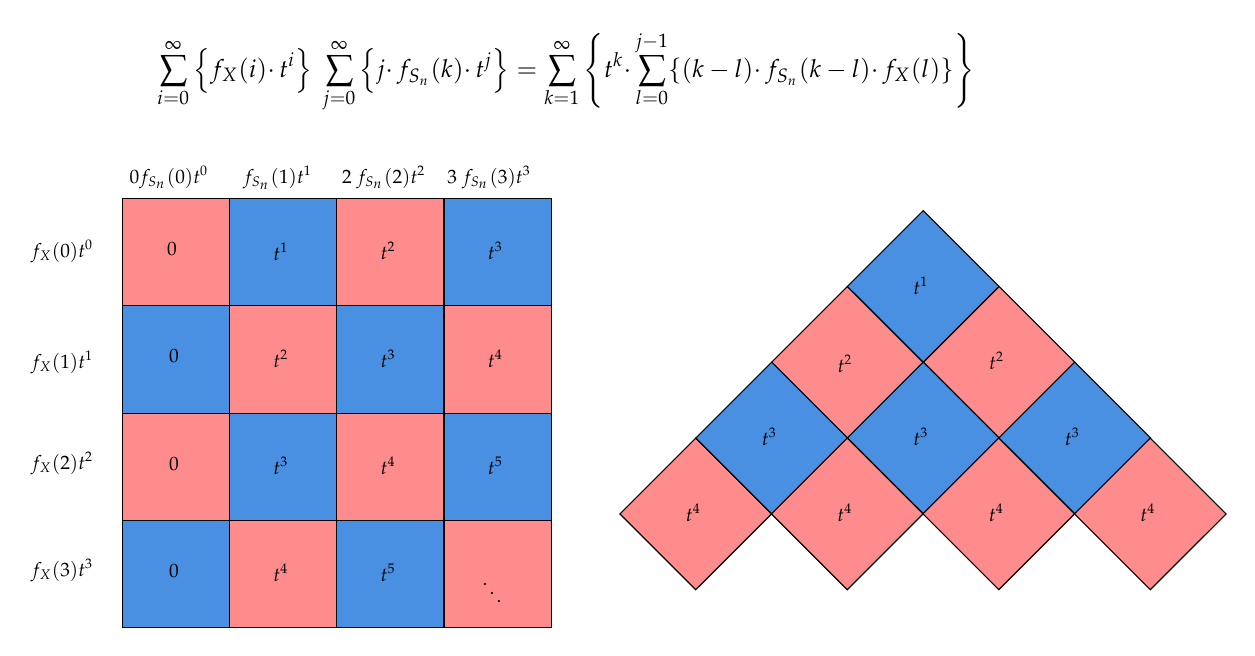
\begin{tikzpicture}[x=0.75pt,y=0.75pt,yscale=-1,xscale=1]
%uncomment if require: \path (0,357); %set diagram left start at 0, and has height of 357

%Shape: Rectangle [id:dp9012494168801195] 
\draw  [color={rgb, 255:red, 0; green, 0; blue, 0 }  ,draw opacity=1 ][fill={rgb, 255:red, 255; green, 140; blue, 140 }  ,fill opacity=1 ] (55.42,87.13) -- (107.08,87.13) -- (107.08,138.8) -- (55.42,138.8) -- cycle ;
%Shape: Rectangle [id:dp13205821049614785] 
\draw  [color={rgb, 255:red, 0; green, 0; blue, 0 }  ,draw opacity=1 ][fill={rgb, 255:red, 255; green, 140; blue, 140 }  ,fill opacity=1 ] (107.08,138.8) -- (158.75,138.8) -- (158.75,190.46) -- (107.08,190.46) -- cycle ;
%Shape: Rectangle [id:dp019003840010249684] 
\draw  [color={rgb, 255:red, 0; green, 0; blue, 0 }  ,draw opacity=1 ][fill={rgb, 255:red, 255; green, 140; blue, 140 }  ,fill opacity=1 ] (158.75,190.46) -- (210.42,190.46) -- (210.42,242.13) -- (158.75,242.13) -- cycle ;
%Shape: Rectangle [id:dp8073038960439742] 
\draw  [color={rgb, 255:red, 0; green, 0; blue, 0 }  ,draw opacity=1 ][fill={rgb, 255:red, 255; green, 140; blue, 140 }  ,fill opacity=1 ] (210.42,242.13) -- (262.09,242.13) -- (262.09,293.8) -- (210.42,293.8) -- cycle ;
%Shape: Rectangle [id:dp417233184317795] 
\draw  [color={rgb, 255:red, 0; green, 0; blue, 0 }  ,draw opacity=1 ][fill={rgb, 255:red, 255; green, 140; blue, 140 }  ,fill opacity=1 ] (210.42,138.8) -- (262.09,138.8) -- (262.09,190.46) -- (210.42,190.46) -- cycle ;
%Shape: Rectangle [id:dp4717191293138612] 
\draw  [color={rgb, 255:red, 0; green, 0; blue, 0 }  ,draw opacity=1 ][fill={rgb, 255:red, 255; green, 140; blue, 140 }  ,fill opacity=1 ] (107.08,242.13) -- (158.75,242.13) -- (158.75,293.8) -- (107.08,293.8) -- cycle ;
%Shape: Rectangle [id:dp13464262358803225] 
\draw  [color={rgb, 255:red, 0; green, 0; blue, 0 }  ,draw opacity=1 ][fill={rgb, 255:red, 255; green, 140; blue, 140 }  ,fill opacity=1 ] (55.42,190.46) -- (107.08,190.46) -- (107.08,242.13) -- (55.42,242.13) -- cycle ;
%Shape: Rectangle [id:dp16637855029421478] 
\draw  [color={rgb, 255:red, 0; green, 0; blue, 0 }  ,draw opacity=1 ][fill={rgb, 255:red, 255; green, 140; blue, 140 }  ,fill opacity=1 ] (158.75,87.13) -- (210.42,87.13) -- (210.42,138.8) -- (158.75,138.8) -- cycle ;

%Shape: Rectangle [id:dp610153790892501] 
\draw  [color={rgb, 255:red, 0; green, 0; blue, 0 }  ,draw opacity=1 ][fill={rgb, 255:red, 74; green, 144; blue, 226 }  ,fill opacity=1 ] (107.08,87.13) -- (158.75,87.13) -- (158.75,138.8) -- (107.08,138.8) -- cycle ;
%Shape: Rectangle [id:dp6072589436516438] 
\draw  [color={rgb, 255:red, 0; green, 0; blue, 0 }  ,draw opacity=1 ][fill={rgb, 255:red, 74; green, 144; blue, 226 }  ,fill opacity=1 ] (55.42,138.8) -- (107.08,138.8) -- (107.08,190.46) -- (55.42,190.46) -- cycle ;
%Shape: Rectangle [id:dp780046034963563] 
\draw  [color={rgb, 255:red, 0; green, 0; blue, 0 }  ,draw opacity=1 ][fill={rgb, 255:red, 74; green, 144; blue, 226 }  ,fill opacity=1 ] (107.08,190.46) -- (158.75,190.46) -- (158.75,242.13) -- (107.08,242.13) -- cycle ;
%Shape: Rectangle [id:dp7830217768491039] 
\draw  [color={rgb, 255:red, 0; green, 0; blue, 0 }  ,draw opacity=1 ][fill={rgb, 255:red, 74; green, 144; blue, 226 }  ,fill opacity=1 ] (55.42,242.13) -- (107.08,242.13) -- (107.08,293.8) -- (55.42,293.8) -- cycle ;
%Shape: Rectangle [id:dp31001434819096274] 
\draw  [color={rgb, 255:red, 0; green, 0; blue, 0 }  ,draw opacity=1 ][fill={rgb, 255:red, 74; green, 144; blue, 226 }  ,fill opacity=1 ] (158.75,138.8) -- (210.42,138.8) -- (210.42,190.46) -- (158.75,190.46) -- cycle ;
%Shape: Rectangle [id:dp44510593714460733] 
\draw  [color={rgb, 255:red, 0; green, 0; blue, 0 }  ,draw opacity=1 ][fill={rgb, 255:red, 74; green, 144; blue, 226 }  ,fill opacity=1 ] (210.42,87.13) -- (262.09,87.13) -- (262.09,138.8) -- (210.42,138.8) -- cycle ;
%Shape: Rectangle [id:dp8059448778013303] 
\draw  [color={rgb, 255:red, 0; green, 0; blue, 0 }  ,draw opacity=1 ][fill={rgb, 255:red, 74; green, 144; blue, 226 }  ,fill opacity=1 ] (158.75,242.13) -- (210.42,242.13) -- (210.42,293.8) -- (158.75,293.8) -- cycle ;
%Shape: Rectangle [id:dp2648498855708319] 
\draw  [color={rgb, 255:red, 0; green, 0; blue, 0 }  ,draw opacity=1 ][fill={rgb, 255:red, 74; green, 144; blue, 226 }  ,fill opacity=1 ] (210.42,190.46) -- (262.09,190.46) -- (262.09,242.13) -- (210.42,242.13) -- cycle ;
%Shape: Rectangle [id:dp3178359683590004] 
\draw  [color={rgb, 255:red, 0; green, 0; blue, 0 }  ,draw opacity=1 ][fill={rgb, 255:red, 255; green, 140; blue, 140 }  ,fill opacity=1 ] (404.75,129.4) -- (441.29,165.93) -- (404.75,202.46) -- (368.22,165.93) -- cycle ;
%Shape: Rectangle [id:dp8097615203830828] 
\draw  [color={rgb, 255:red, 0; green, 0; blue, 0 }  ,draw opacity=1 ][fill={rgb, 255:red, 255; green, 140; blue, 140 }  ,fill opacity=1 ] (331.68,202.46) -- (368.22,239) -- (331.68,275.53) -- (295.15,239) -- cycle ;
%Shape: Rectangle [id:dp6579946521796063] 
\draw  [color={rgb, 255:red, 0; green, 0; blue, 0 }  ,draw opacity=1 ][fill={rgb, 255:red, 255; green, 140; blue, 140 }  ,fill opacity=1 ] (477.82,129.4) -- (514.36,165.93) -- (477.82,202.46) -- (441.29,165.93) -- cycle ;
%Shape: Rectangle [id:dp1676638549029934] 
\draw  [color={rgb, 255:red, 0; green, 0; blue, 0 }  ,draw opacity=1 ][fill={rgb, 255:red, 74; green, 144; blue, 226 }  ,fill opacity=1 ] (441.29,92.86) -- (477.82,129.4) -- (441.29,165.93) -- (404.75,129.4) -- cycle ;
%Shape: Rectangle [id:dp8681065944365156] 
\draw  [color={rgb, 255:red, 0; green, 0; blue, 0 }  ,draw opacity=1 ][fill={rgb, 255:red, 74; green, 144; blue, 226 }  ,fill opacity=1 ] (368.29,165.86) -- (404.82,202.4) -- (368.29,238.93) -- (331.75,202.4) -- cycle ;
%Shape: Rectangle [id:dp655906660349328] 
\draw  [color={rgb, 255:red, 0; green, 0; blue, 0 }  ,draw opacity=1 ][fill={rgb, 255:red, 74; green, 144; blue, 226 }  ,fill opacity=1 ] (441.29,165.86) -- (477.82,202.4) -- (441.29,238.93) -- (404.75,202.4) -- cycle ;
%Shape: Rectangle [id:dp08139212530978601] 
\draw  [color={rgb, 255:red, 0; green, 0; blue, 0 }  ,draw opacity=1 ][fill={rgb, 255:red, 74; green, 144; blue, 226 }  ,fill opacity=1 ] (514.29,165.86) -- (550.82,202.4) -- (514.29,238.93) -- (477.75,202.4) -- cycle ;
%Shape: Rectangle [id:dp4420360995937358] 
\draw  [color={rgb, 255:red, 0; green, 0; blue, 0 }  ,draw opacity=1 ][fill={rgb, 255:red, 255; green, 140; blue, 140 }  ,fill opacity=1 ] (404.68,202.46) -- (441.22,239) -- (404.68,275.53) -- (368.15,239) -- cycle ;
%Shape: Rectangle [id:dp766503793931888] 
\draw  [color={rgb, 255:red, 0; green, 0; blue, 0 }  ,draw opacity=1 ][fill={rgb, 255:red, 255; green, 140; blue, 140 }  ,fill opacity=1 ] (477.68,202.46) -- (514.22,239) -- (477.68,275.53) -- (441.15,239) -- cycle ;
%Shape: Rectangle [id:dp5853286419881494] 
\draw  [color={rgb, 255:red, 0; green, 0; blue, 0 }  ,draw opacity=1 ][fill={rgb, 255:red, 255; green, 140; blue, 140 }  ,fill opacity=1 ] (550.68,202.46) -- (587.22,239) -- (550.68,275.53) -- (514.15,239) -- cycle ;

% Text Node
\draw (71,5) node [anchor=north west][inner sep=0.75pt]  [font=\small] [align=left] {$\displaystyle \sum ^{\infty }_{i=0}\left\{f_{X}( i) \cdotp t^{i}\right\} \ \sum ^{\infty }_{j=0}\left\{j\cdotp f_{S_{n}}( k) \cdotp t^{j}\right\} =\sum ^{\infty }_{k=1}\left\{t^{k} \cdotp \sum ^{j-1}_{l=0}\{( k-l) \cdotp f_{S_{n}}( k-l) \cdotp f_{X}( l)\}\right\}$};
% Text Node
\draw (57.7,70.2) node [anchor=north west][inner sep=0.75pt]  [font=\scriptsize] [align=left] {$\displaystyle 0f_{S_{n}}( 0) t^{0}$};
% Text Node
\draw (112.37,70.2) node [anchor=north west][inner sep=0.75pt]  [font=\scriptsize] [align=left] {$\displaystyle f_{S_{n}}( 1) t^{1}$};
% Text Node
\draw (160.04,70.2) node [anchor=north west][inner sep=0.75pt]  [font=\scriptsize] [align=left] {$\displaystyle 2\ f_{S_{n}}( 2) t^{2}$};
% Text Node
\draw (10.08,105.6) node [anchor=north west][inner sep=0.75pt]  [font=\scriptsize] [align=left] {$\displaystyle f_{X}( 0) t^{0}$};
% Text Node
\draw (10.08,159.08) node [anchor=north west][inner sep=0.75pt]  [font=\scriptsize] [align=left] {$\displaystyle f_{X}( 1) t^{1}$};
% Text Node
\draw (10.08,208.03) node [anchor=north west][inner sep=0.75pt]  [font=\scriptsize] [align=left] {$\displaystyle f_{X}( 2) t^{2}$};
% Text Node
\draw (10.08,259.7) node [anchor=north west][inner sep=0.75pt]  [font=\scriptsize] [align=left] {$\displaystyle f_{X}( 3) t^{3}$};
% Text Node
\draw (210.8,70.2) node [anchor=north west][inner sep=0.75pt]  [font=\scriptsize] [align=left] {$\displaystyle 3\ f_{S_{n}}( 3) t^{3}$};
% Text Node
\draw (126.92,158.63) node [anchor=north west][inner sep=0.75pt]  [font=\scriptsize] [align=left] {$\displaystyle t^{2}$};
% Text Node
\draw (126.92,106.96) node [anchor=north west][inner sep=0.75pt]  [font=\scriptsize] [align=left] {$\displaystyle t^{1}$};
% Text Node
\draw (178.59,106.96) node [anchor=north west][inner sep=0.75pt]  [font=\scriptsize] [align=left] {$\displaystyle t^{2}$};
% Text Node
\draw (76.66,261.97) node [anchor=north west][inner sep=0.75pt]  [font=\scriptsize] [align=left] {$\displaystyle 0$};
% Text Node
\draw (76.66,210.3) node [anchor=north west][inner sep=0.75pt]  [font=\scriptsize] [align=left] {$\displaystyle 0$};
% Text Node
\draw (76.66,158.63) node [anchor=north west][inner sep=0.75pt]  [font=\scriptsize] [align=left] {$\displaystyle 0$};
% Text Node
\draw (75.75,106.96) node [anchor=north west][inner sep=0.75pt]  [font=\scriptsize] [align=left] {$\displaystyle 0$};
% Text Node
\draw (126.92,210.3) node [anchor=north west][inner sep=0.75pt]  [font=\scriptsize] [align=left] {$\displaystyle t^{3}$};
% Text Node
\draw (178.59,158.63) node [anchor=north west][inner sep=0.75pt]  [font=\scriptsize] [align=left] {$\displaystyle t^{3}$};
% Text Node
\draw (230.25,106.96) node [anchor=north west][inner sep=0.75pt]  [font=\scriptsize] [align=left] {$\displaystyle t^{3}$};
% Text Node
\draw (230.25,158.63) node [anchor=north west][inner sep=0.75pt]  [font=\scriptsize] [align=left] {$\displaystyle t^{4}$};
% Text Node
\draw (178.59,210.3) node [anchor=north west][inner sep=0.75pt]  [font=\scriptsize] [align=left] {$\displaystyle t^{4}$};
% Text Node
\draw (126.92,261.97) node [anchor=north west][inner sep=0.75pt]  [font=\scriptsize] [align=left] {$\displaystyle t^{4}$};
% Text Node
\draw (178.59,261.97) node [anchor=north west][inner sep=0.75pt]  [font=\scriptsize] [align=left] {$\displaystyle t^{5}$};
% Text Node
\draw (230.25,210.3) node [anchor=north west][inner sep=0.75pt]  [font=\scriptsize] [align=left] {$\displaystyle t^{5}$};
% Text Node
\draw (227.25,261.97) node [anchor=north west][inner sep=0.75pt]  [font=\scriptsize] [align=left] {$\displaystyle \ddots $};
% Text Node
\draw (435.29,123.4) node [anchor=north west][inner sep=0.75pt]  [font=\scriptsize] [align=left] {$\displaystyle t^{1}$};
% Text Node
\draw (362.29,196.4) node [anchor=north west][inner sep=0.75pt]  [font=\scriptsize] [align=left] {$\displaystyle t^{3}$};
% Text Node
\draw (435.29,196.4) node [anchor=north west][inner sep=0.75pt]  [font=\scriptsize] [align=left] {$\displaystyle t^{3}$};
% Text Node
\draw (508.29,196.4) node [anchor=north west][inner sep=0.75pt]  [font=\scriptsize] [align=left] {$\displaystyle t^{3}$};
% Text Node
\draw (398.75,161.4) node [anchor=north west][inner sep=0.75pt]  [font=\scriptsize] [align=left] {$\displaystyle t^{2}$};
% Text Node
\draw (471.82,159.93) node [anchor=north west][inner sep=0.75pt]  [font=\scriptsize] [align=left] {$\displaystyle t^{2}$};
% Text Node
\draw (325.68,233) node [anchor=north west][inner sep=0.75pt]  [font=\scriptsize] [align=left] {$\displaystyle t^{4}$};
% Text Node
\draw (398.68,233) node [anchor=north west][inner sep=0.75pt]  [font=\scriptsize] [align=left] {$\displaystyle t^{4}$};
% Text Node
\draw (471.68,233) node [anchor=north west][inner sep=0.75pt]  [font=\scriptsize] [align=left] {$\displaystyle t^{4}$};
% Text Node
\draw (544.68,233) node [anchor=north west][inner sep=0.75pt]  [font=\scriptsize] [align=left] {$\displaystyle t^{4}$};
\end{tikzpicture}

\end{center}



\end{multicols*}
\end{document}


